% Options for packages loaded elsewhere
\PassOptionsToPackage{unicode}{hyperref}
\PassOptionsToPackage{hyphens}{url}
\PassOptionsToPackage{dvipsnames,svgnames,x11names}{xcolor}
%
\documentclass[
  letterpaper,
  DIV=11,
  numbers=noendperiod]{scrartcl}

\usepackage{amsmath,amssymb}
\usepackage{iftex}
\ifPDFTeX
  \usepackage[T1]{fontenc}
  \usepackage[utf8]{inputenc}
  \usepackage{textcomp} % provide euro and other symbols
\else % if luatex or xetex
  \usepackage{unicode-math}
  \defaultfontfeatures{Scale=MatchLowercase}
  \defaultfontfeatures[\rmfamily]{Ligatures=TeX,Scale=1}
\fi
\usepackage{lmodern}
\ifPDFTeX\else  
    % xetex/luatex font selection
\fi
% Use upquote if available, for straight quotes in verbatim environments
\IfFileExists{upquote.sty}{\usepackage{upquote}}{}
\IfFileExists{microtype.sty}{% use microtype if available
  \usepackage[]{microtype}
  \UseMicrotypeSet[protrusion]{basicmath} % disable protrusion for tt fonts
}{}
\makeatletter
\@ifundefined{KOMAClassName}{% if non-KOMA class
  \IfFileExists{parskip.sty}{%
    \usepackage{parskip}
  }{% else
    \setlength{\parindent}{0pt}
    \setlength{\parskip}{6pt plus 2pt minus 1pt}}
}{% if KOMA class
  \KOMAoptions{parskip=half}}
\makeatother
\usepackage{xcolor}
\setlength{\emergencystretch}{3em} % prevent overfull lines
\setcounter{secnumdepth}{-\maxdimen} % remove section numbering
% Make \paragraph and \subparagraph free-standing
\makeatletter
\ifx\paragraph\undefined\else
  \let\oldparagraph\paragraph
  \renewcommand{\paragraph}{
    \@ifstar
      \xxxParagraphStar
      \xxxParagraphNoStar
  }
  \newcommand{\xxxParagraphStar}[1]{\oldparagraph*{#1}\mbox{}}
  \newcommand{\xxxParagraphNoStar}[1]{\oldparagraph{#1}\mbox{}}
\fi
\ifx\subparagraph\undefined\else
  \let\oldsubparagraph\subparagraph
  \renewcommand{\subparagraph}{
    \@ifstar
      \xxxSubParagraphStar
      \xxxSubParagraphNoStar
  }
  \newcommand{\xxxSubParagraphStar}[1]{\oldsubparagraph*{#1}\mbox{}}
  \newcommand{\xxxSubParagraphNoStar}[1]{\oldsubparagraph{#1}\mbox{}}
\fi
\makeatother

\usepackage{color}
\usepackage{fancyvrb}
\newcommand{\VerbBar}{|}
\newcommand{\VERB}{\Verb[commandchars=\\\{\}]}
\DefineVerbatimEnvironment{Highlighting}{Verbatim}{commandchars=\\\{\}}
% Add ',fontsize=\small' for more characters per line
\usepackage{framed}
\definecolor{shadecolor}{RGB}{241,243,245}
\newenvironment{Shaded}{\begin{snugshade}}{\end{snugshade}}
\newcommand{\AlertTok}[1]{\textcolor[rgb]{0.68,0.00,0.00}{#1}}
\newcommand{\AnnotationTok}[1]{\textcolor[rgb]{0.37,0.37,0.37}{#1}}
\newcommand{\AttributeTok}[1]{\textcolor[rgb]{0.40,0.45,0.13}{#1}}
\newcommand{\BaseNTok}[1]{\textcolor[rgb]{0.68,0.00,0.00}{#1}}
\newcommand{\BuiltInTok}[1]{\textcolor[rgb]{0.00,0.23,0.31}{#1}}
\newcommand{\CharTok}[1]{\textcolor[rgb]{0.13,0.47,0.30}{#1}}
\newcommand{\CommentTok}[1]{\textcolor[rgb]{0.37,0.37,0.37}{#1}}
\newcommand{\CommentVarTok}[1]{\textcolor[rgb]{0.37,0.37,0.37}{\textit{#1}}}
\newcommand{\ConstantTok}[1]{\textcolor[rgb]{0.56,0.35,0.01}{#1}}
\newcommand{\ControlFlowTok}[1]{\textcolor[rgb]{0.00,0.23,0.31}{\textbf{#1}}}
\newcommand{\DataTypeTok}[1]{\textcolor[rgb]{0.68,0.00,0.00}{#1}}
\newcommand{\DecValTok}[1]{\textcolor[rgb]{0.68,0.00,0.00}{#1}}
\newcommand{\DocumentationTok}[1]{\textcolor[rgb]{0.37,0.37,0.37}{\textit{#1}}}
\newcommand{\ErrorTok}[1]{\textcolor[rgb]{0.68,0.00,0.00}{#1}}
\newcommand{\ExtensionTok}[1]{\textcolor[rgb]{0.00,0.23,0.31}{#1}}
\newcommand{\FloatTok}[1]{\textcolor[rgb]{0.68,0.00,0.00}{#1}}
\newcommand{\FunctionTok}[1]{\textcolor[rgb]{0.28,0.35,0.67}{#1}}
\newcommand{\ImportTok}[1]{\textcolor[rgb]{0.00,0.46,0.62}{#1}}
\newcommand{\InformationTok}[1]{\textcolor[rgb]{0.37,0.37,0.37}{#1}}
\newcommand{\KeywordTok}[1]{\textcolor[rgb]{0.00,0.23,0.31}{\textbf{#1}}}
\newcommand{\NormalTok}[1]{\textcolor[rgb]{0.00,0.23,0.31}{#1}}
\newcommand{\OperatorTok}[1]{\textcolor[rgb]{0.37,0.37,0.37}{#1}}
\newcommand{\OtherTok}[1]{\textcolor[rgb]{0.00,0.23,0.31}{#1}}
\newcommand{\PreprocessorTok}[1]{\textcolor[rgb]{0.68,0.00,0.00}{#1}}
\newcommand{\RegionMarkerTok}[1]{\textcolor[rgb]{0.00,0.23,0.31}{#1}}
\newcommand{\SpecialCharTok}[1]{\textcolor[rgb]{0.37,0.37,0.37}{#1}}
\newcommand{\SpecialStringTok}[1]{\textcolor[rgb]{0.13,0.47,0.30}{#1}}
\newcommand{\StringTok}[1]{\textcolor[rgb]{0.13,0.47,0.30}{#1}}
\newcommand{\VariableTok}[1]{\textcolor[rgb]{0.07,0.07,0.07}{#1}}
\newcommand{\VerbatimStringTok}[1]{\textcolor[rgb]{0.13,0.47,0.30}{#1}}
\newcommand{\WarningTok}[1]{\textcolor[rgb]{0.37,0.37,0.37}{\textit{#1}}}

\providecommand{\tightlist}{%
  \setlength{\itemsep}{0pt}\setlength{\parskip}{0pt}}\usepackage{longtable,booktabs,array}
\usepackage{calc} % for calculating minipage widths
% Correct order of tables after \paragraph or \subparagraph
\usepackage{etoolbox}
\makeatletter
\patchcmd\longtable{\par}{\if@noskipsec\mbox{}\fi\par}{}{}
\makeatother
% Allow footnotes in longtable head/foot
\IfFileExists{footnotehyper.sty}{\usepackage{footnotehyper}}{\usepackage{footnote}}
\makesavenoteenv{longtable}
\usepackage{graphicx}
\makeatletter
\def\maxwidth{\ifdim\Gin@nat@width>\linewidth\linewidth\else\Gin@nat@width\fi}
\def\maxheight{\ifdim\Gin@nat@height>\textheight\textheight\else\Gin@nat@height\fi}
\makeatother
% Scale images if necessary, so that they will not overflow the page
% margins by default, and it is still possible to overwrite the defaults
% using explicit options in \includegraphics[width, height, ...]{}
\setkeys{Gin}{width=\maxwidth,height=\maxheight,keepaspectratio}
% Set default figure placement to htbp
\makeatletter
\def\fps@figure{htbp}
\makeatother
% definitions for citeproc citations
\NewDocumentCommand\citeproctext{}{}
\NewDocumentCommand\citeproc{mm}{%
  \begingroup\def\citeproctext{#2}\cite{#1}\endgroup}
\makeatletter
 % allow citations to break across lines
 \let\@cite@ofmt\@firstofone
 % avoid brackets around text for \cite:
 \def\@biblabel#1{}
 \def\@cite#1#2{{#1\if@tempswa , #2\fi}}
\makeatother
\newlength{\cslhangindent}
\setlength{\cslhangindent}{1.5em}
\newlength{\csllabelwidth}
\setlength{\csllabelwidth}{3em}
\newenvironment{CSLReferences}[2] % #1 hanging-indent, #2 entry-spacing
 {\begin{list}{}{%
  \setlength{\itemindent}{0pt}
  \setlength{\leftmargin}{0pt}
  \setlength{\parsep}{0pt}
  % turn on hanging indent if param 1 is 1
  \ifodd #1
   \setlength{\leftmargin}{\cslhangindent}
   \setlength{\itemindent}{-1\cslhangindent}
  \fi
  % set entry spacing
  \setlength{\itemsep}{#2\baselineskip}}}
 {\end{list}}
\usepackage{calc}
\newcommand{\CSLBlock}[1]{\hfill\break\parbox[t]{\linewidth}{\strut\ignorespaces#1\strut}}
\newcommand{\CSLLeftMargin}[1]{\parbox[t]{\csllabelwidth}{\strut#1\strut}}
\newcommand{\CSLRightInline}[1]{\parbox[t]{\linewidth - \csllabelwidth}{\strut#1\strut}}
\newcommand{\CSLIndent}[1]{\hspace{\cslhangindent}#1}

\KOMAoption{captions}{tableheading}
\makeatletter
\@ifpackageloaded{caption}{}{\usepackage{caption}}
\AtBeginDocument{%
\ifdefined\contentsname
  \renewcommand*\contentsname{Table of contents}
\else
  \newcommand\contentsname{Table of contents}
\fi
\ifdefined\listfigurename
  \renewcommand*\listfigurename{List of Figures}
\else
  \newcommand\listfigurename{List of Figures}
\fi
\ifdefined\listtablename
  \renewcommand*\listtablename{List of Tables}
\else
  \newcommand\listtablename{List of Tables}
\fi
\ifdefined\figurename
  \renewcommand*\figurename{Figure}
\else
  \newcommand\figurename{Figure}
\fi
\ifdefined\tablename
  \renewcommand*\tablename{Table}
\else
  \newcommand\tablename{Table}
\fi
}
\@ifpackageloaded{float}{}{\usepackage{float}}
\floatstyle{ruled}
\@ifundefined{c@chapter}{\newfloat{codelisting}{h}{lop}}{\newfloat{codelisting}{h}{lop}[chapter]}
\floatname{codelisting}{Listing}
\newcommand*\listoflistings{\listof{codelisting}{List of Listings}}
\makeatother
\makeatletter
\makeatother
\makeatletter
\@ifpackageloaded{caption}{}{\usepackage{caption}}
\@ifpackageloaded{subcaption}{}{\usepackage{subcaption}}
\makeatother

\ifLuaTeX
  \usepackage{selnolig}  % disable illegal ligatures
\fi
\usepackage{bookmark}

\IfFileExists{xurl.sty}{\usepackage{xurl}}{} % add URL line breaks if available
\urlstyle{same} % disable monospaced font for URLs
\hypersetup{
  pdftitle={Beyond the Surface},
  pdfauthor={Tyler Wiederich},
  colorlinks=true,
  linkcolor={blue},
  filecolor={Maroon},
  citecolor={Blue},
  urlcolor={Blue},
  pdfcreator={LaTeX via pandoc}}


\title{Beyond the Surface}
\usepackage{etoolbox}
\makeatletter
\providecommand{\subtitle}[1]{% add subtitle to \maketitle
  \apptocmd{\@title}{\par {\large #1 \par}}{}{}
}
\makeatother
\subtitle{Evaluating Perception and Accuracy in 3D Printed Data
Visualizations}
\author{Tyler Wiederich}
\date{September 29, 2025}

\begin{document}
\maketitle


\subsection{Overview}\label{overview}

\begin{itemize}
\tightlist
\item
  Motivation and Background
\item
  Roadmap
\item
  Projects

  \begin{enumerate}
  \def\labelenumi{\arabic{enumi}.}
  \tightlist
  \item
    3D Bar Charts
  \item
    Experiential Learning
  \item
    3D Heat Maps
  \end{enumerate}
\item
  Contribution
\end{itemize}

Experiential learning serves a dual purpose by letting Stat 218 students
interact with the study, thus letting us get a large sample size

\begin{Shaded}
\begin{Highlighting}[]
\FunctionTok{library}\NormalTok{(tidyverse)}
\end{Highlighting}
\end{Shaded}

\begin{verbatim}
-- Attaching core tidyverse packages ------------------------ tidyverse 2.0.0 --
v dplyr     1.1.4     v readr     2.1.5
v forcats   1.0.0     v stringr   1.5.2
v ggplot2   4.0.0     v tibble    3.3.0
v lubridate 1.9.4     v tidyr     1.3.1
v purrr     1.1.0     
-- Conflicts ------------------------------------------ tidyverse_conflicts() --
x dplyr::filter() masks stats::filter()
x dplyr::lag()    masks stats::lag()
i Use the conflicted package (<http://conflicted.r-lib.org/>) to force all conflicts to become errors
\end{verbatim}

\section{Motivation}\label{motivation}

\subsection{Motivation}\label{motivation-1}

Modern statistical graphics exist largely within the confines of 2D
projections.

\begin{itemize}
\tightlist
\item
  Research articles
\item
  Textbooks
\item
  Documentation / reports
\item
  News articles
\end{itemize}

Why?

\begin{itemize}
\tightlist
\item
  Easy to make / understand
\item
  Low cost to produce
\item
  Many available software options
\end{itemize}

\begin{figure}[H]

{\centering 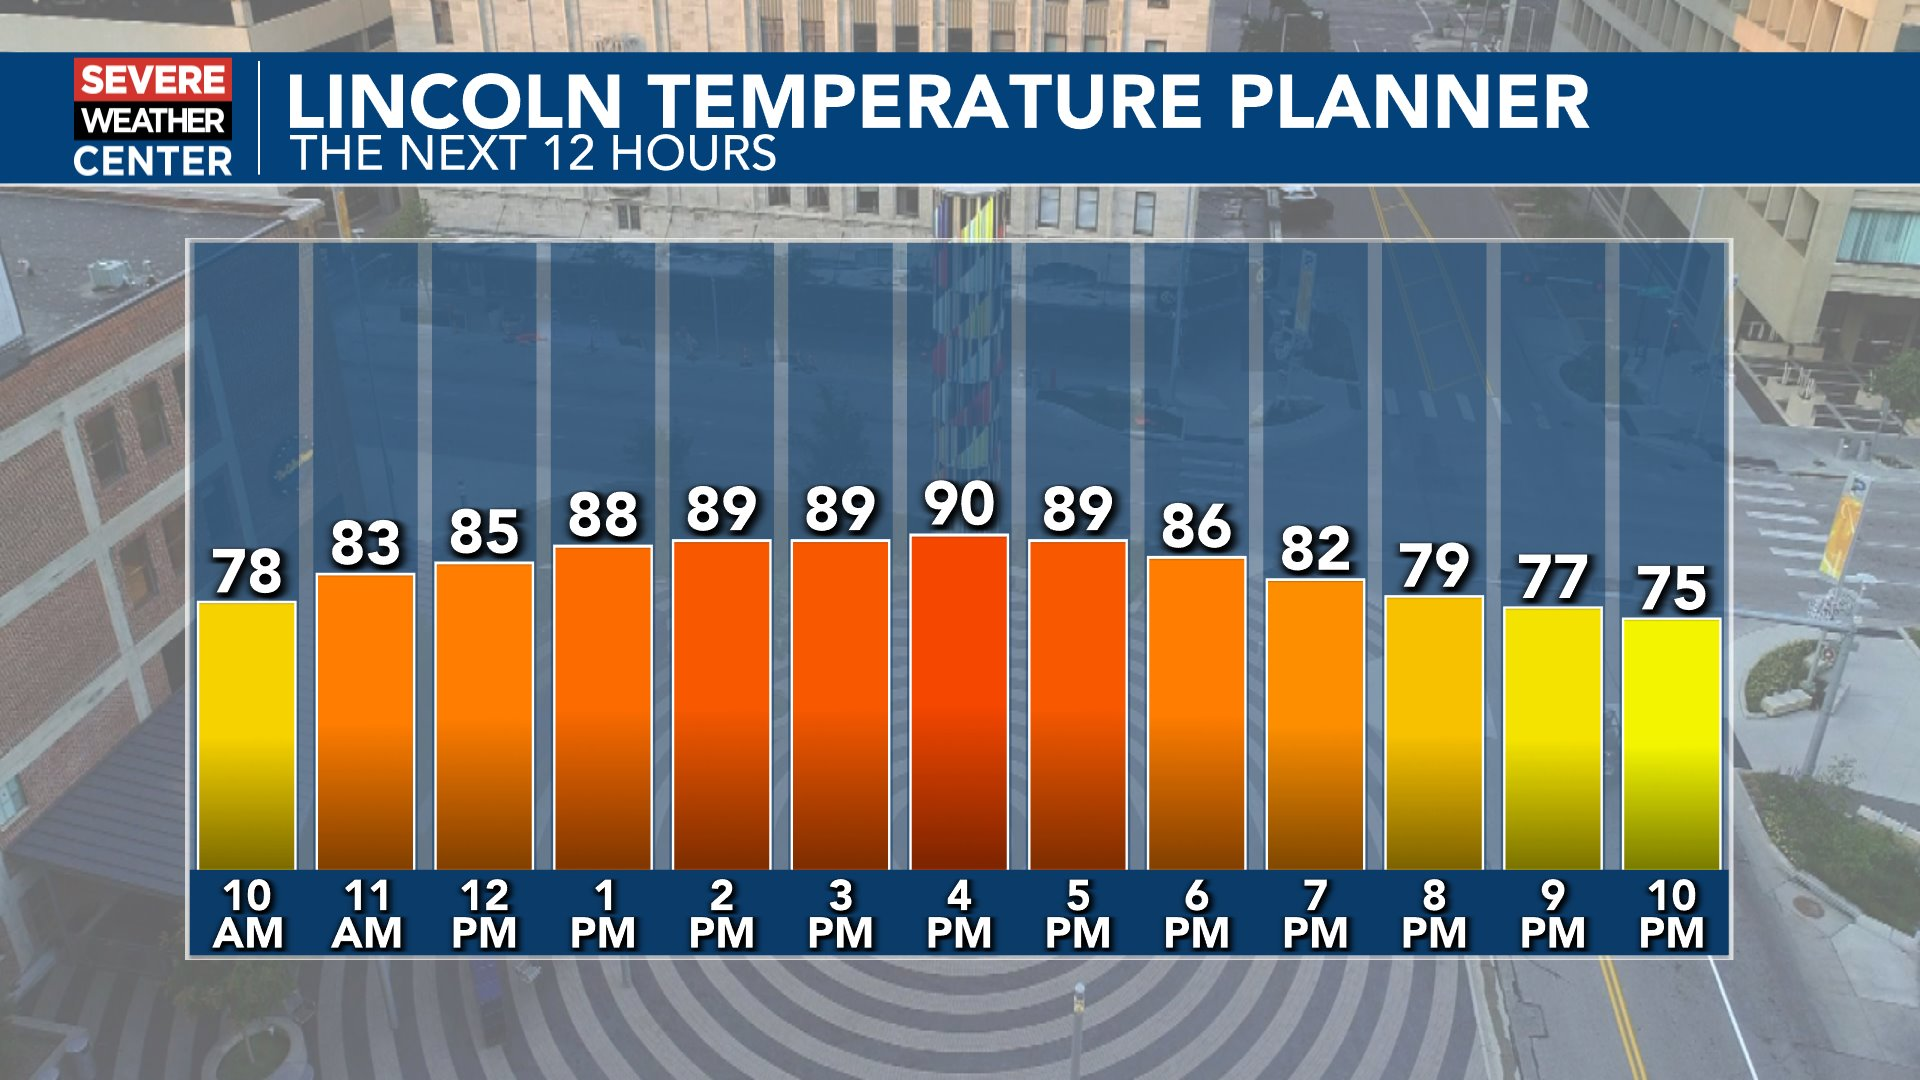
\includegraphics[width=0.5\textwidth,height=\textheight]{images/koln-weather.jpg}

}

\caption{\emph{Source: www.1011now.com}}

\end{figure}%%
\begin{figure}[H]

{\centering 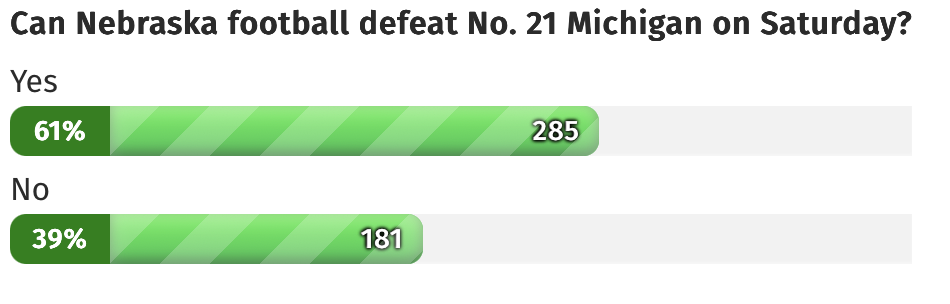
\includegraphics[width=0.5\textwidth,height=\textheight]{images/klkntv-poll.png}

}

\caption{\emph{Source: www.klkntv.com}}

\end{figure}%%
\begin{figure}[H]

{\centering 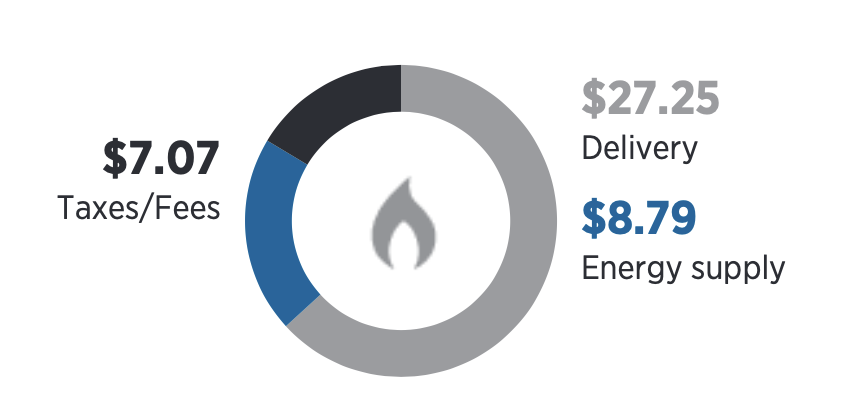
\includegraphics[width=0.5\textwidth,height=\textheight]{images/blackhills-energy-bill.png}

}

\caption{\emph{Source: Black Hills Energy}}

\end{figure}%

\subsection{Motivation}\label{motivation-2}

The rise in computer graphics also included the pioneering of 3D
graphical renderings \footnote{Armstrong (2016)} \footnote{Murdoch and
  Adler (2024)}. Many software programs include options for creating
such charts, including:

\begin{itemize}
\tightlist
\item
  R
\item
  Python
\item
  SAS
\item
  MATLAB
\item
  SPSS
\item
  etc.
\end{itemize}

\begin{figure}

\centering{

\includegraphics{images/rotating-penguins.gif}

}

\caption{\label{fig-rotating-scatter}3D scatterplot of the Palmer
Penguins dataset from Horst, Hill, and Gorman (2020)}

\end{figure}%

Mention Excel in the list of software

The first digital 3d software was Sketchpad, created by Ivan Sutherland
as part of his PhD in 1963.

\begin{center}\rule{0.5\linewidth}{0.5pt}\end{center}

\begin{figure}

\begin{minipage}{0.50\linewidth}

\centering{

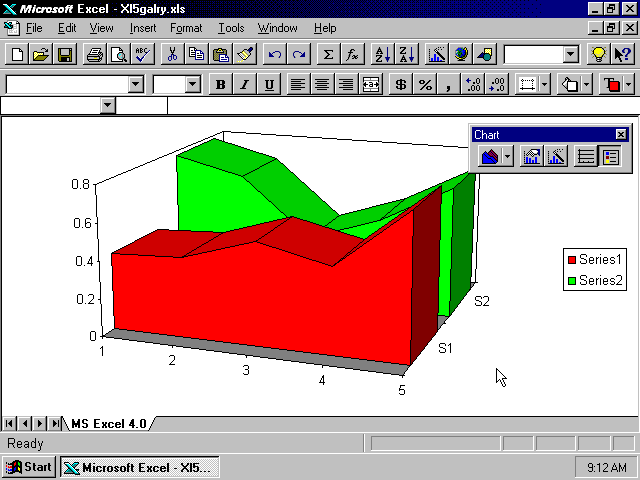
\includegraphics[width=\textwidth,height=4.16667in]{images/excel95-3d-chart.png}

}

\subcaption{\label{fig-excel3}Microsoft® Excel 95}

\end{minipage}%
%
\begin{minipage}{0.50\linewidth}

\centering{

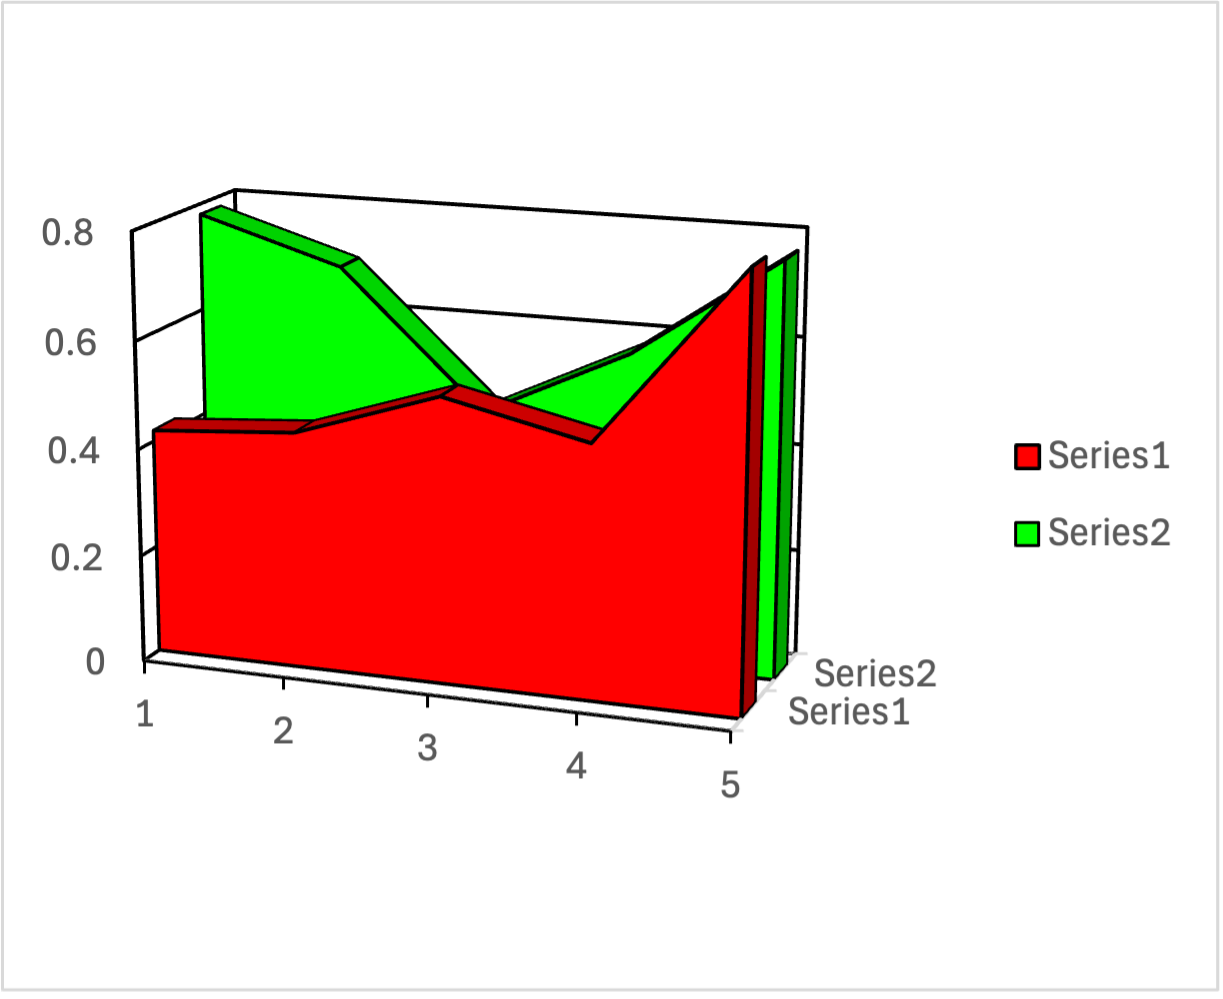
\includegraphics[width=\textwidth,height=4.16667in]{images/excel-modern-surface.png}

}

\subcaption{\label{fig-modern}Microsoft ® Excel for Mac, Version 16}

\end{minipage}%

\caption{\label{fig-excel}Two 3D charts created with Microsoft® Excel}

\end{figure}%

Other types of 3d charts include area, line, bar, and pie

\subsection{Motivation}\label{motivation-3}

To date, there is no widespread usage of 3D statistical graphics outside
of 2D projections. They are generally considered to be items of
interest, without a formal role in data interpretations.

\begin{figure}

\centering{

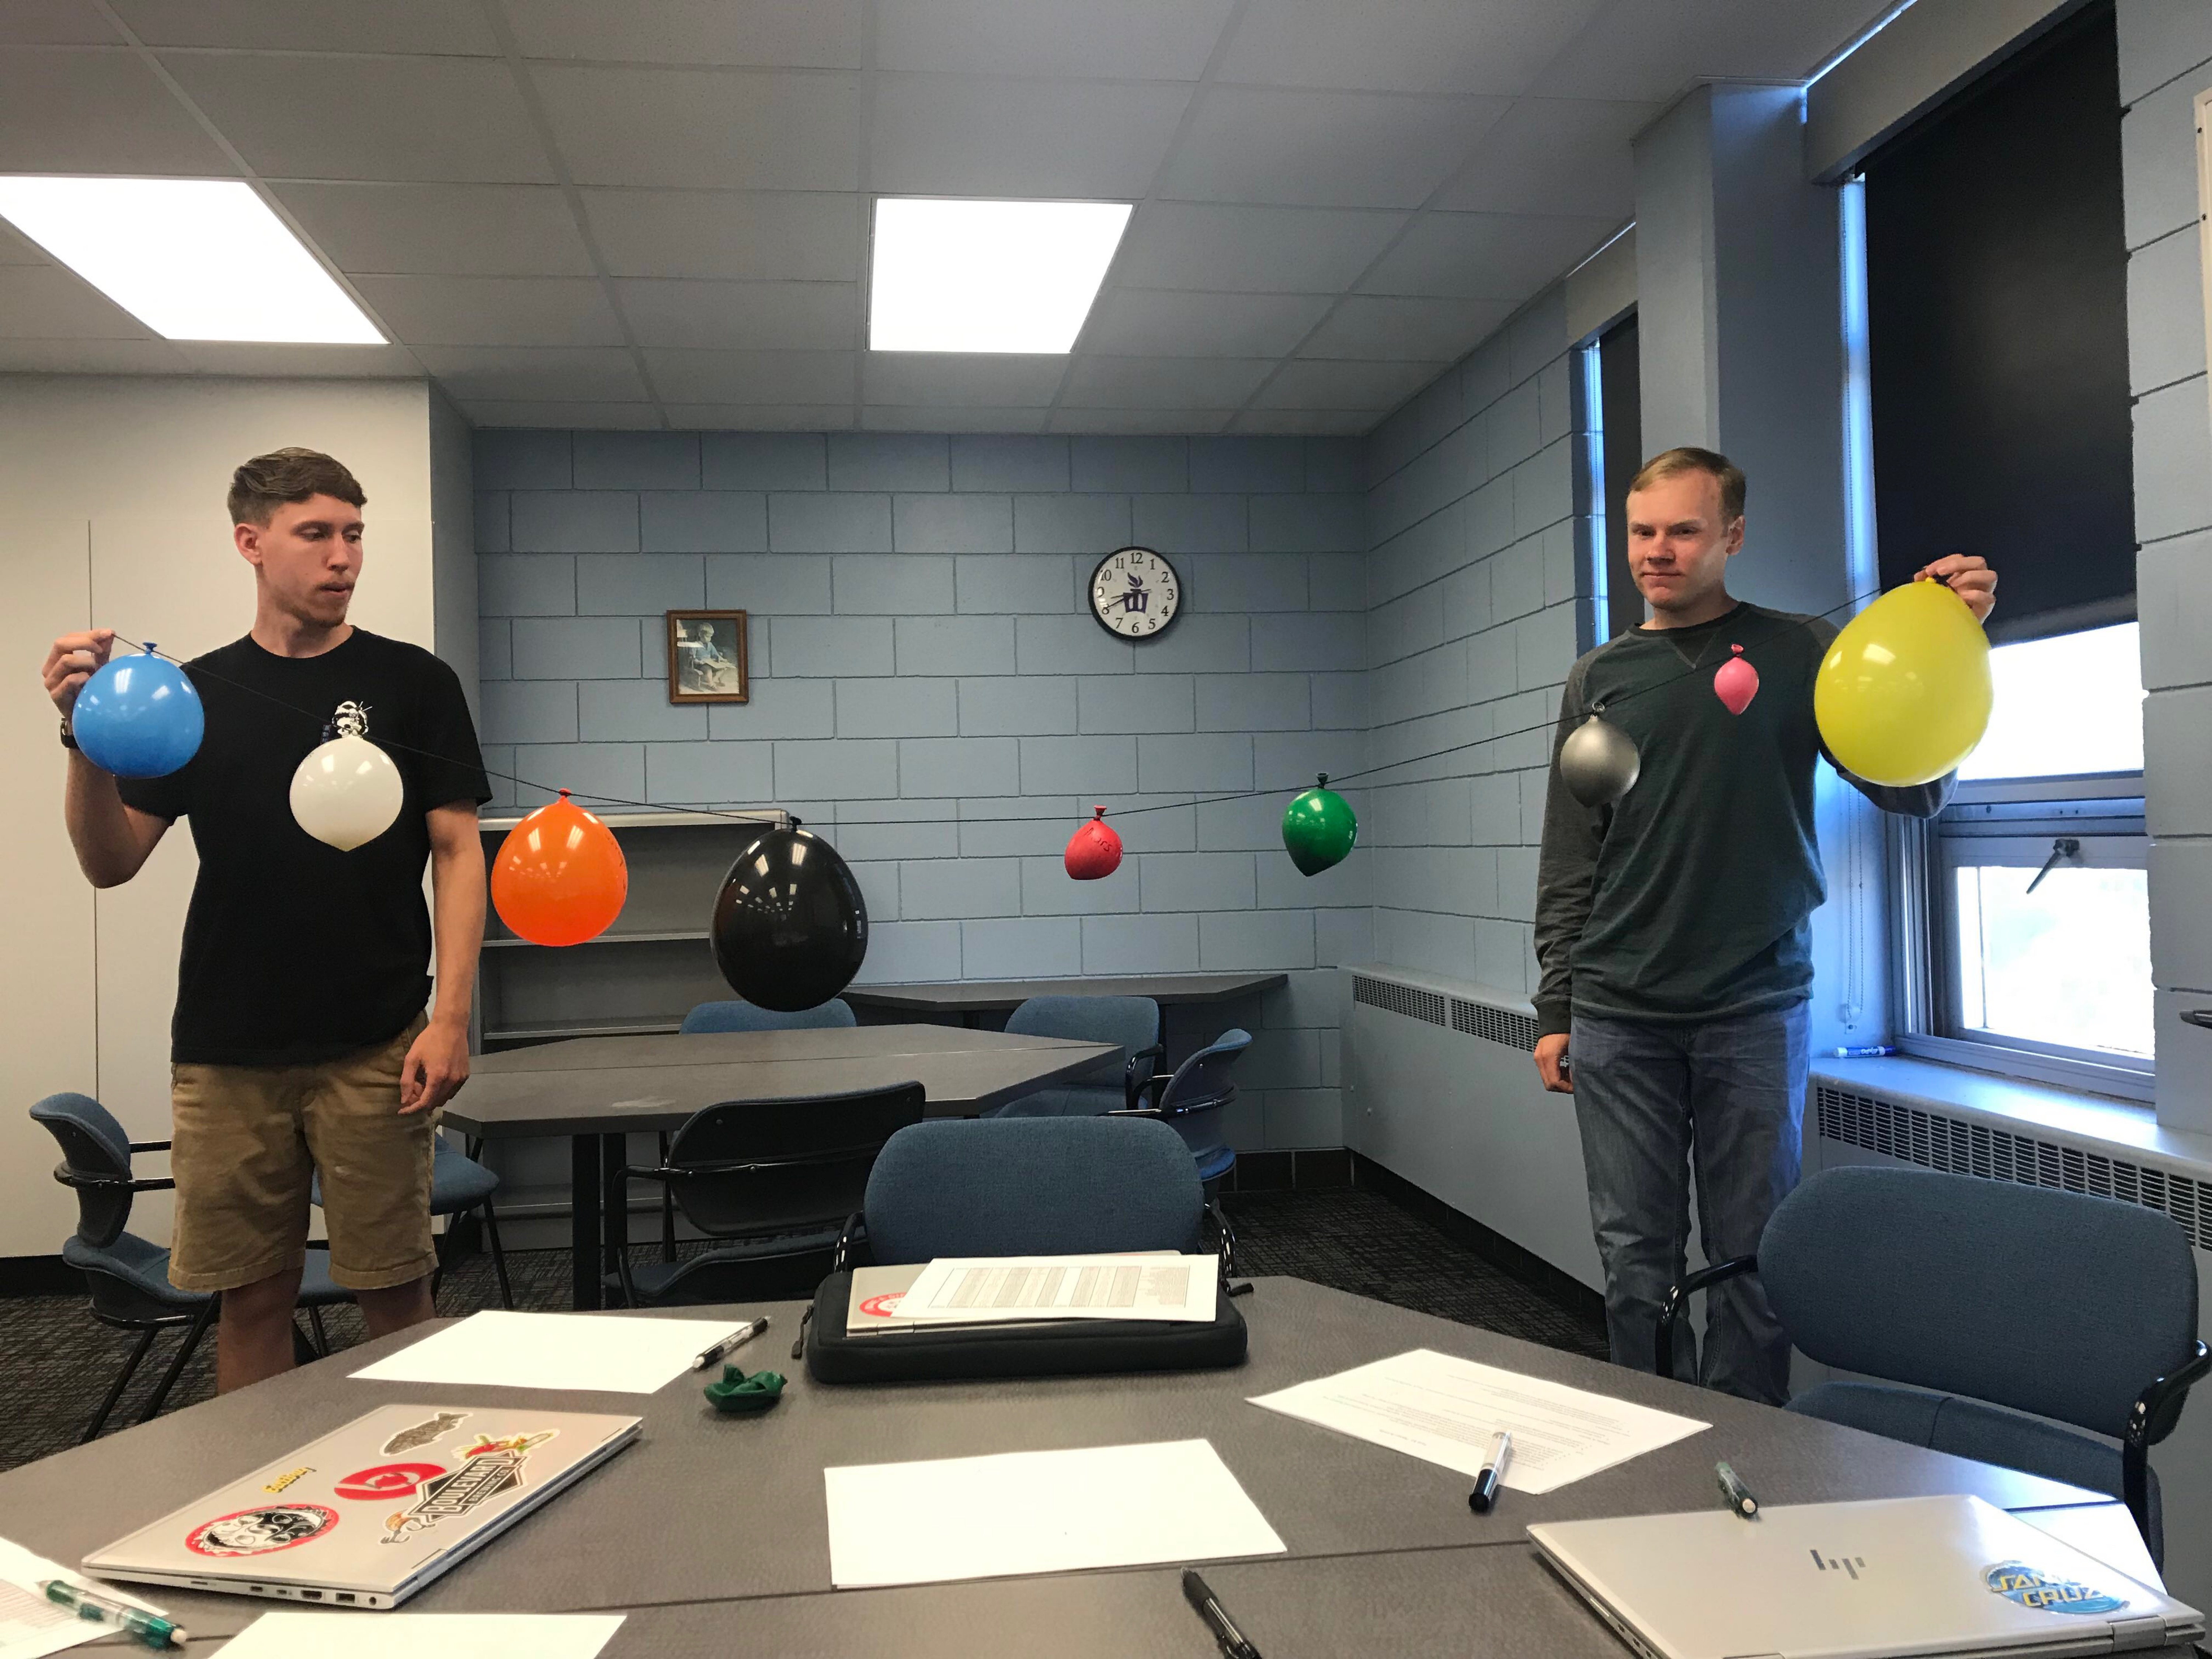
\includegraphics{images/solar-system.JPG}

}

\caption{\label{fig-dsci210}3D visualization of \_\_\_ in DSCI 210 at
Winona State University, 2019.}

\end{figure}%

There are many instances of data physicalization, but often utilized for
unique artistic displays.

\section{Background}\label{background}

\subsection{Evaluation of 3D Charts}\label{evaluation-of-3d-charts}

There are many possible metrics to evaluate the qualities of a chart
\footnote{Vanderplas, Cook, and Hofmann (2020)} \footnote{VanderPlas and
  Hofmann (2017)} \footnote{Buja et al. (2009)} \footnote{Cleveland and
  McGill (1984)} \footnote{Peña, Ragan, and Harrison (2020)}.

\begin{itemize}
\item
  Accuracy
\item
  Response times
\item
  Pattern recognition
\item
  Memorability
\item
  Preference
\end{itemize}

\subsection{Types of 3D charts}\label{types-of-3d-charts}

3D charts can be grouped into one of two categories.

\textbf{Decorative 3D}

\begin{itemize}
\tightlist
\item
  2D charts converted drawn to have artificial axis
\item
  Considered to be ``chart junk''\footnote{Tufte (2001)}
\item
  Static renderings
\end{itemize}

\textbf{Informational 3D}

\begin{itemize}
\tightlist
\item
  All axes convey information
\item
  Intuitive use cases
\item
  Static or interactive renderings
\end{itemize}

\subsection{Data beyond a screen}\label{data-beyond-a-screen}

Many studies on 2D and 3D charts have one key limitation: they are
limited to 3D charts presented on 2D surfaces. With modern technology,
we are able to create 3D charts in our 3D world via 3D-printing. The
rising popularity and decreasing cost of 3D printers makes this option
more feasible to implement in the communication of data.

\begin{figure}

\centering{

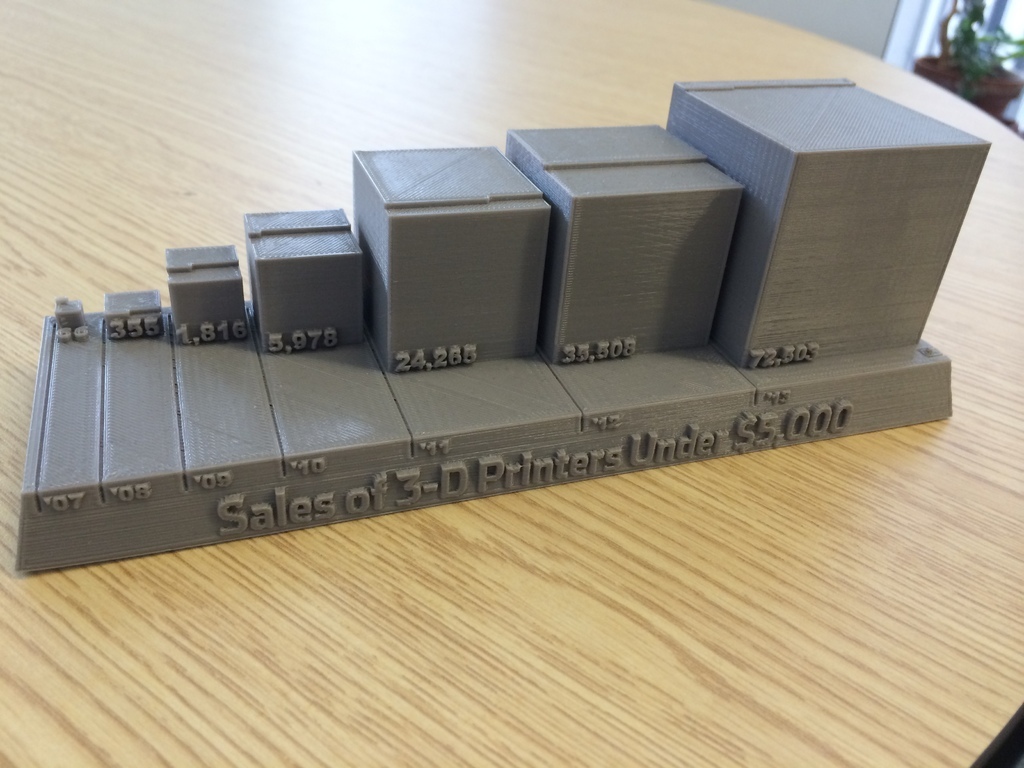
\includegraphics{images/first-3d-printed-chart.jpg}

}

\caption{\label{fig-wsj2014}3D-printed representation of 3D printer
sales. Source: Wall Street Journal
\href{https://www.thingiverse.com/thing:365994}{(link to print)}}

\end{figure}%

\begin{itemize}
\tightlist
\item
  Kraus et al. (2020) uses VR
\end{itemize}

\subsection{Why study 3D-printed
charts?}\label{why-study-3d-printed-charts}

There are several reasons to explore this medium of statistical
graphics.

\begin{itemize}
\tightlist
\item
  Interactions are more natural than digitized counterparts
\item
  Increased recall of information \footnote{Stusak, Schwarz, and Butz
    (2015)} \footnote{Stusak, Hobe, and Butz (2016)}
\item
  Realistic use cases for informational/educational purposes
\end{itemize}

\subsection{Research Objectives}\label{research-objectives}

Data physicalization of statistical graphics has not been widely
studied. In our research, we are broadly studying the following
questions:

\begin{itemize}
\tightlist
\item
  Do 3D-printed charts follow patterns found in previous studies that
  compared different types of charts?
\end{itemize}

\begin{itemize}
\tightlist
\item
  Are 3D-printed charts better or worse than their digitized
  counterparts (2D and 3D renderings) regarding numerical accuracies of
  stimuli ratio comparisons?
\end{itemize}

\begin{itemize}
\tightlist
\item
  How do students participating in our experiments reflect on the
  scientific process, both as a participant and when viewing the study
  through the eyes of a researcher?
\end{itemize}

I believe only there are only a couple of studies that focus on the
memorability of statistical graphics

\subsection{Research Overview}\label{research-overview}

\textbf{Project 1}

\begin{itemize}
\tightlist
\item
  Study of 3D-printed bar charts
\item
  Pilot study within the Statistics department
\end{itemize}

\textbf{Project 2}

\begin{itemize}
\tightlist
\item
  Incorporate the experiment of Project 1 into the curriculum of Stat
  218
\item
  Give students a series of reflections related to the experiment,
  allowing us to follow students from participants to consumers of
  scientific knowledge
\end{itemize}

\textbf{Project 3}

\begin{itemize}
\tightlist
\item
  Same format as Project 2, but replacing the 3D bar charts with 3D heat
  maps
\end{itemize}

\begin{figure}

\begin{minipage}{\linewidth}
~\end{minipage}%
\newline
\begin{minipage}{\linewidth}
\begin{center}
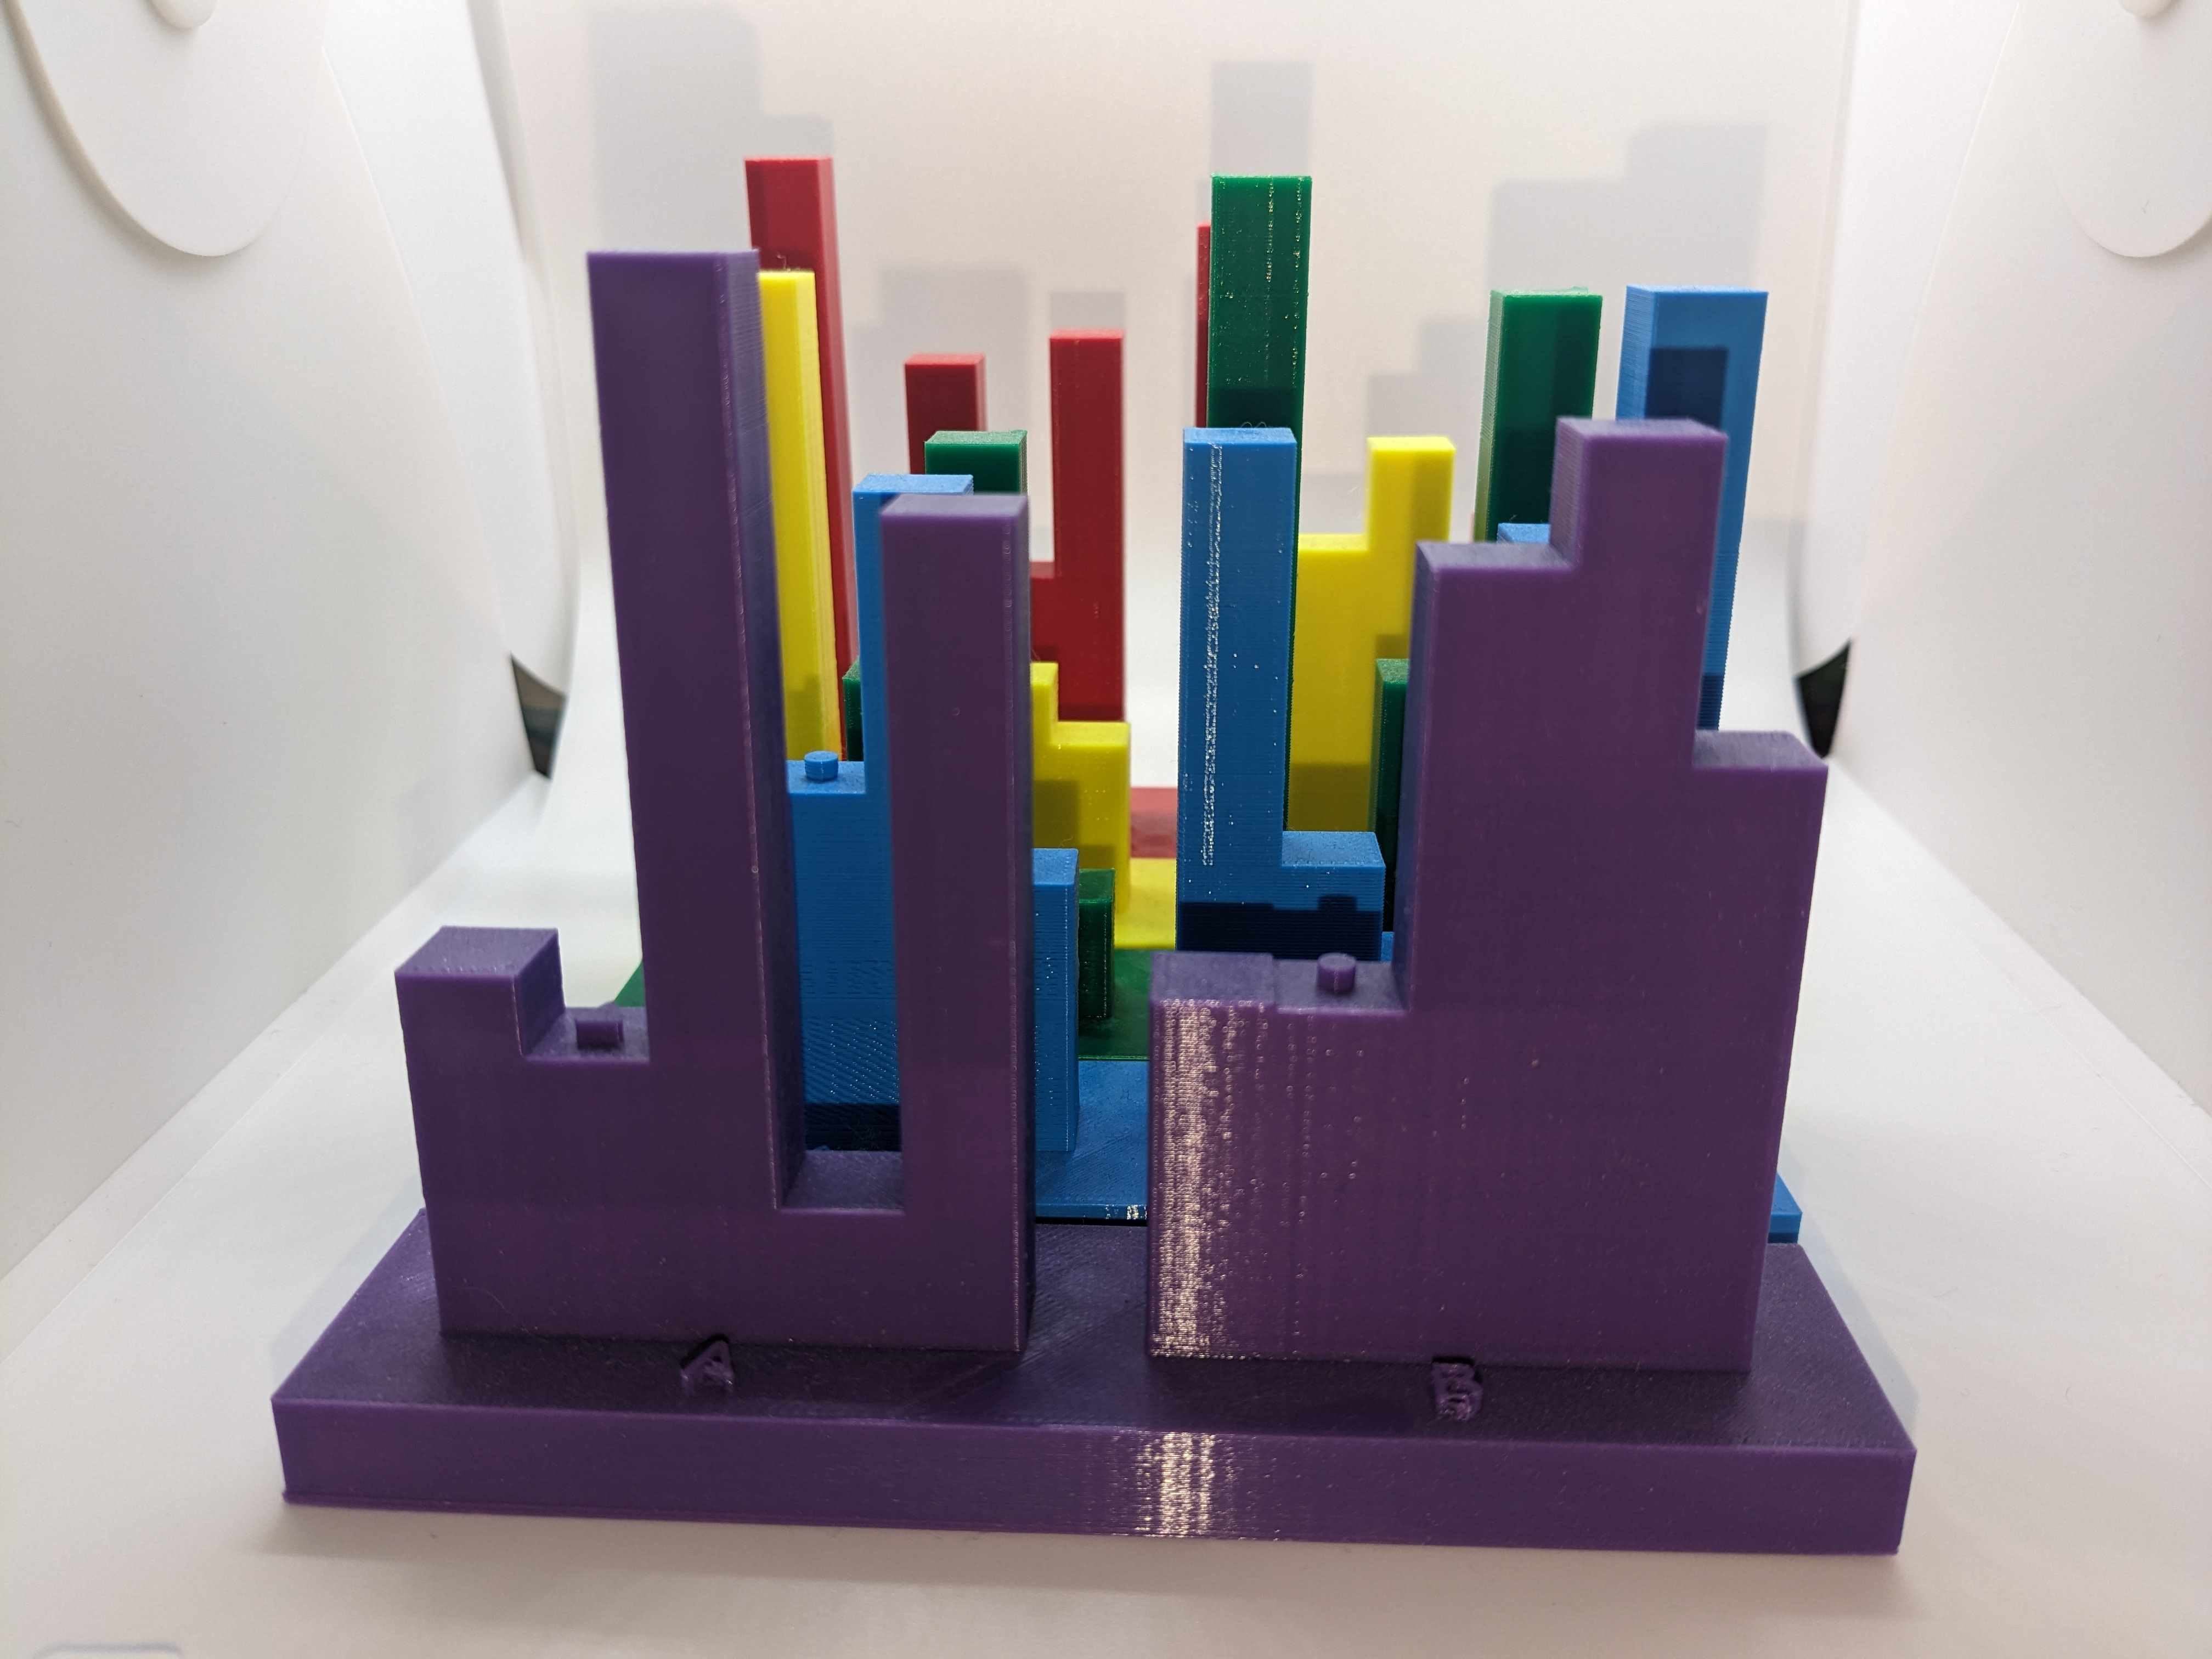
\includegraphics{images/proj1-examp.jpg}
\end{center}
\end{minipage}%

\end{figure}%

\begin{figure}

\begin{minipage}{\linewidth}
~\end{minipage}%
\newline
\begin{minipage}{\linewidth}
\begin{center}
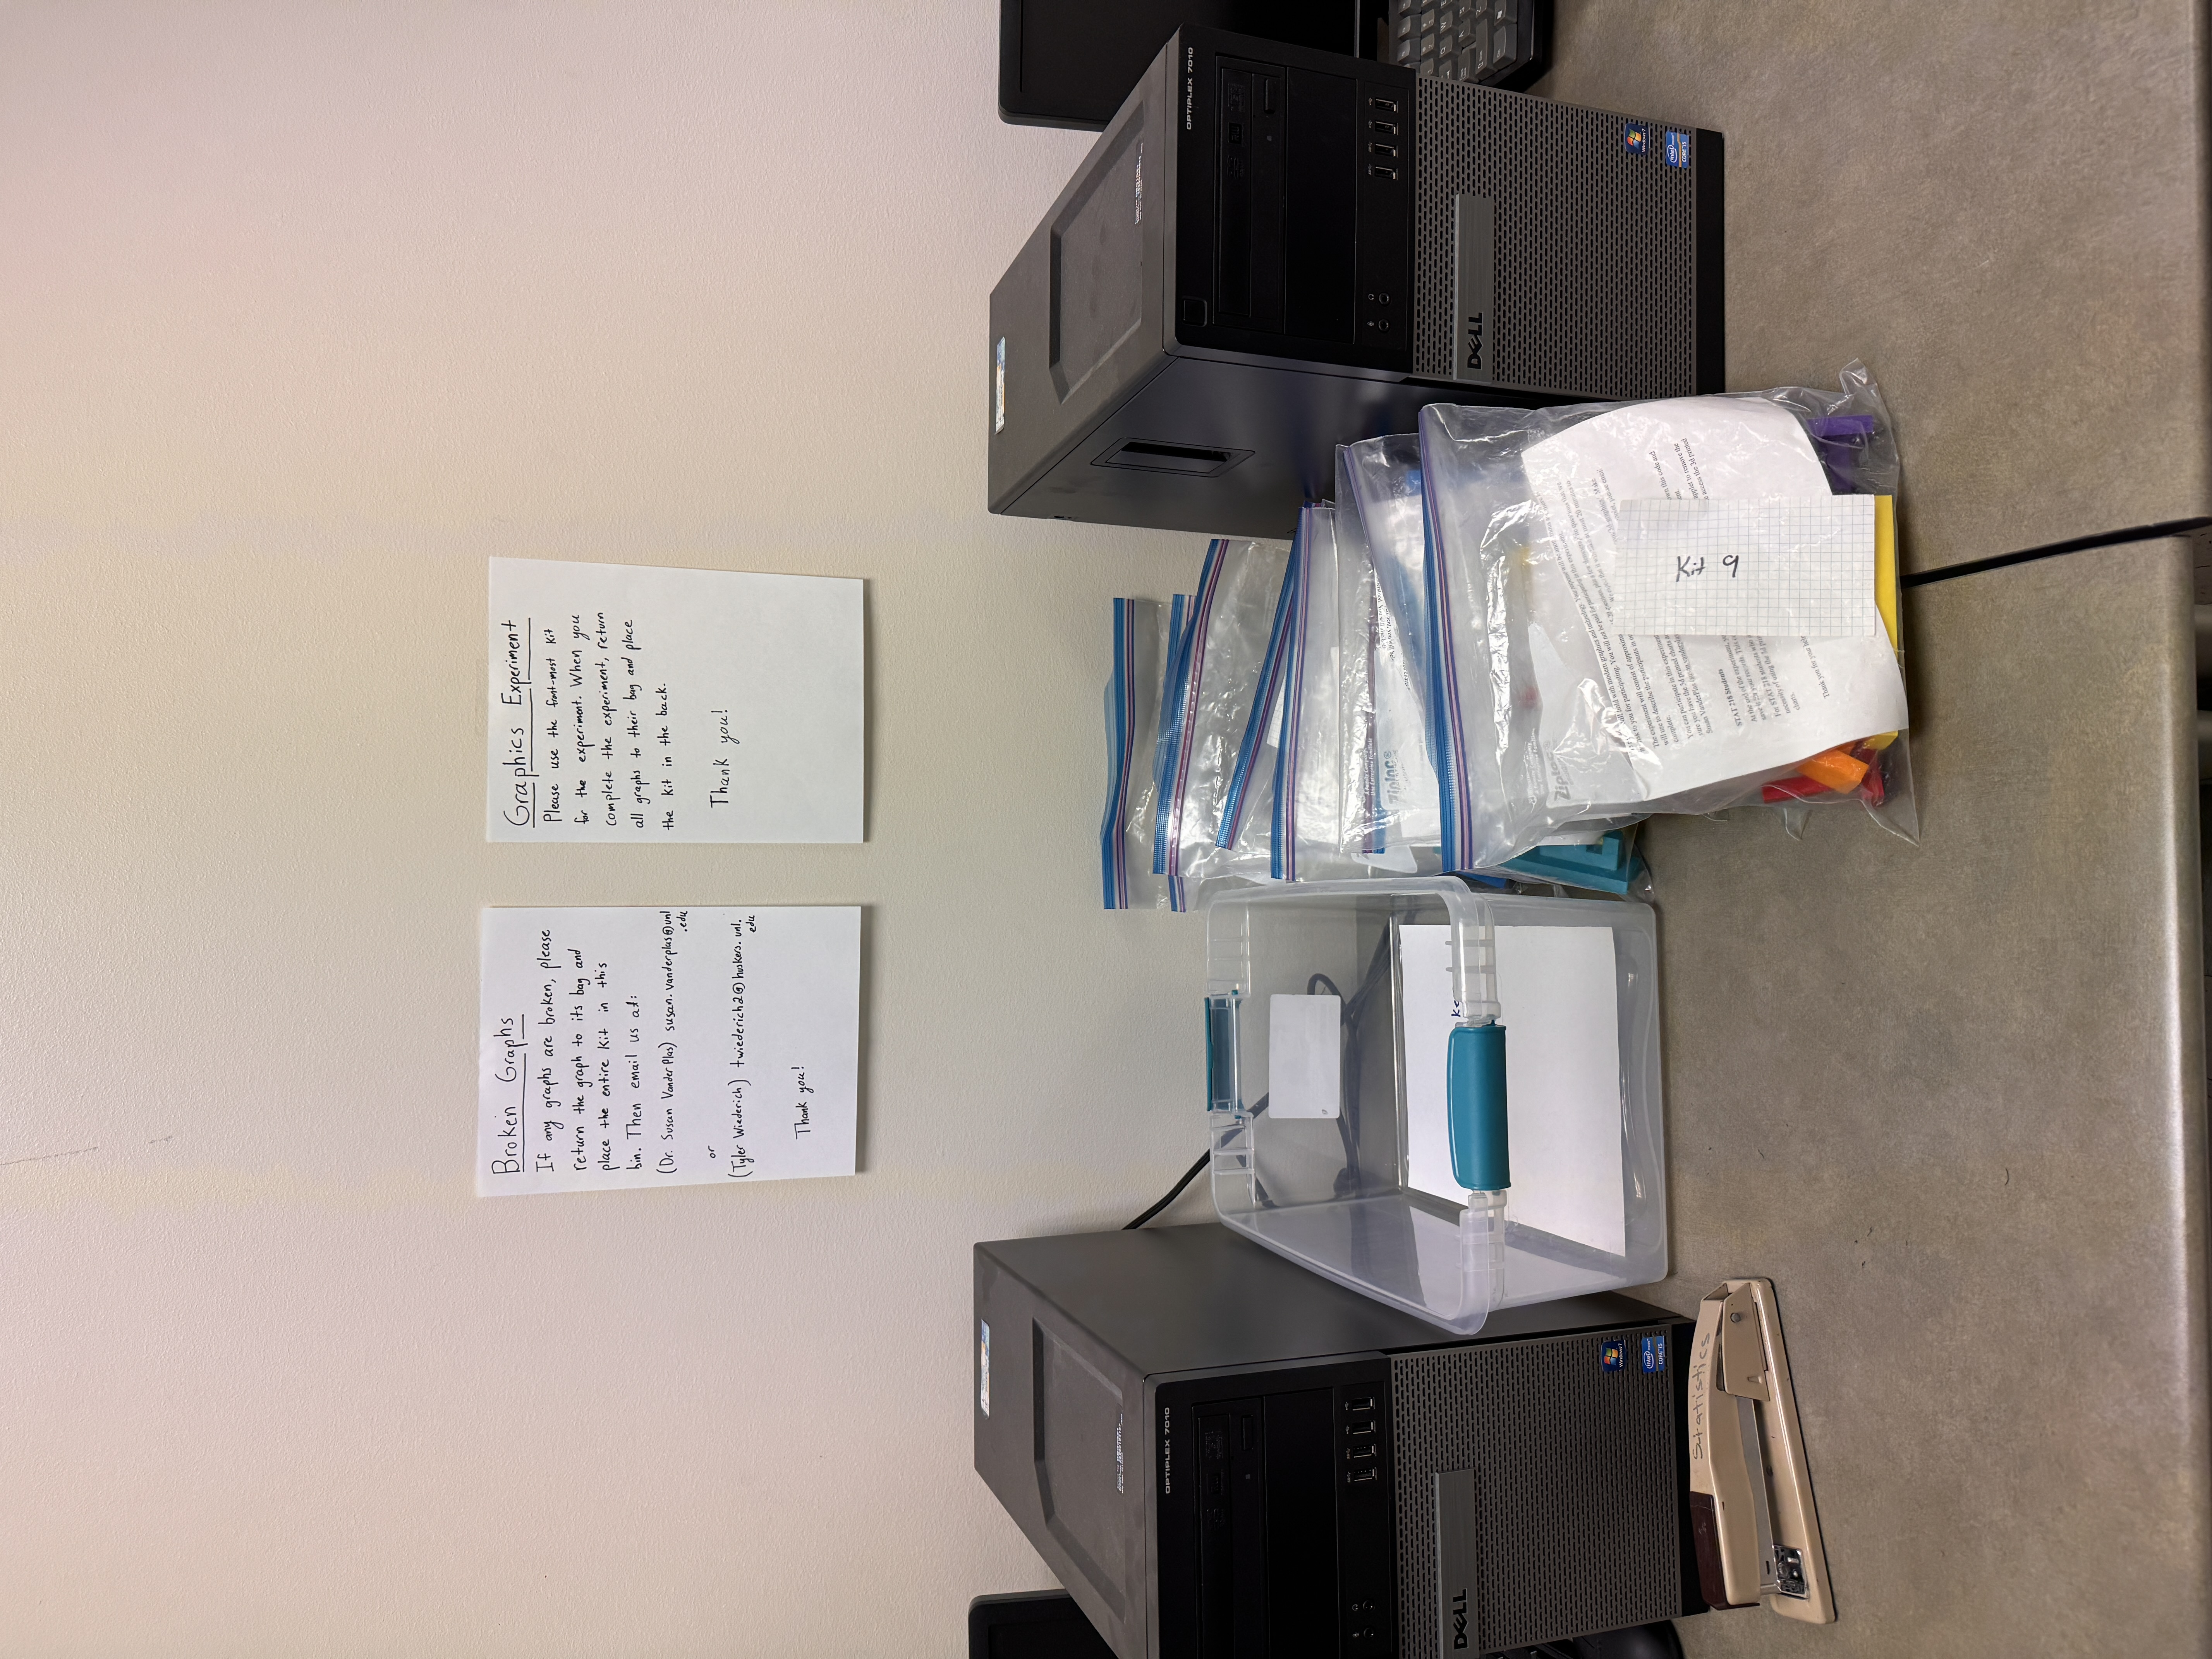
\includegraphics{images/stat218-proj1.JPG}
\end{center}
\end{minipage}%

\end{figure}%

\begin{figure}

\begin{minipage}{\linewidth}
~\end{minipage}%
\newline
\begin{minipage}{\linewidth}
\begin{center}
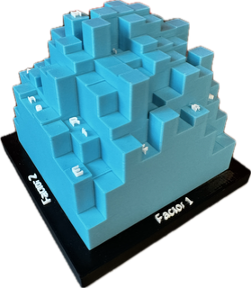
\includegraphics{images/examp3dp.png}
\end{center}
\end{minipage}%

\end{figure}%

\subsection{Roadmap}\label{roadmap}

\textbf{3D Bar Charts}

\begin{itemize}
\tightlist
\item
  ✅ Lit Review
\item
  ✅ Design
\item
  ✅ Data Collection
\item
  ✅ Analysis
\item
  ✅ Write-up
\end{itemize}

\textbf{Experiential Learning}

\begin{itemize}
\tightlist
\item
  ☑️ Lit Review
\item
  ✅ Design
\item
  ➡️ Data Collection

  \begin{itemize}
  \tightlist
  \item
    ✅ 3D Bar Charts
  \item
    ➡️ 3D Heat Maps
  \end{itemize}
\item
  Analysis
\item
  Write-up
\end{itemize}

\textbf{3D Heat Maps}

\begin{itemize}
\tightlist
\item
  ✅ Lit Review
\item
  ✅ Design
\item
  ➡️ Data Collection
\item
  Analysis
\item
  Write-up
\end{itemize}

\section{Project 1: 3D Bar Charts}\label{project-1-3d-bar-charts}

\subsection{3D Bar Charts}\label{d-bar-charts}

\begin{figure}

\begin{minipage}{0.33\linewidth}

\centering{

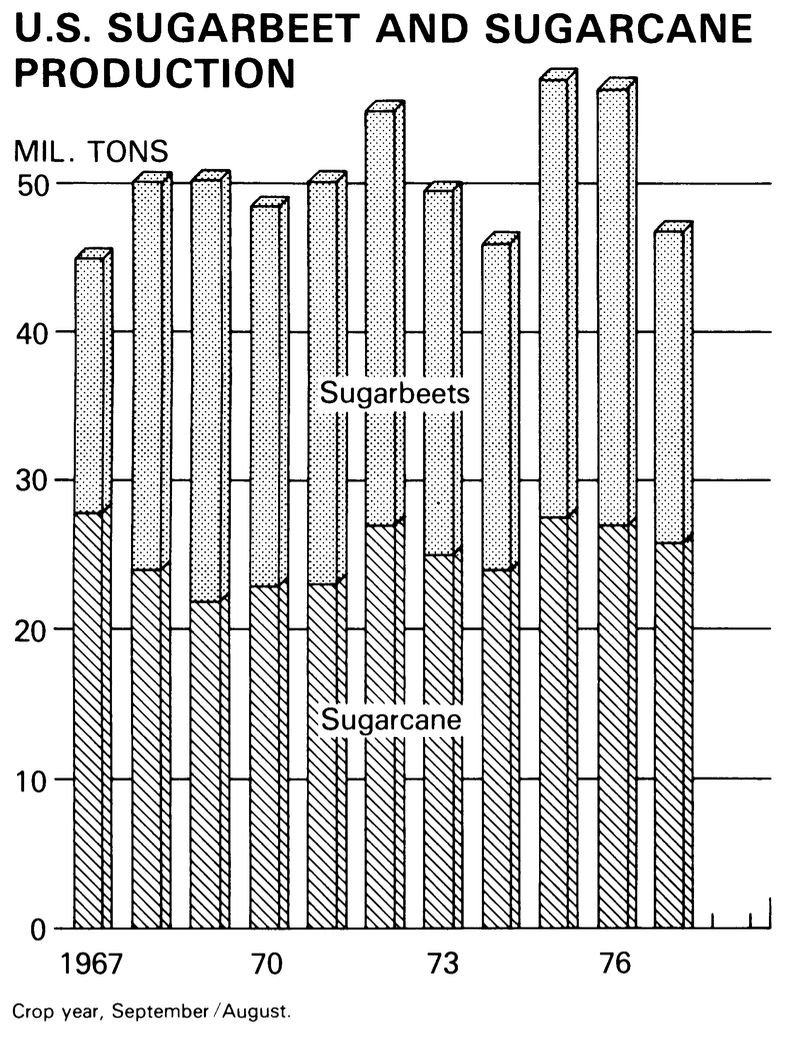
\includegraphics[width=\textwidth,height=4.16667in]{images/preferance-example1.png}

}

\subcaption{\label{fig-examp1}Figure from \emph{1978 Handbook of
Agricultural Charts. Enlargements / {[}u.s. Department of
Agriculture{]}} (1978)}

\end{minipage}%
%
\begin{minipage}{0.33\linewidth}

\centering{

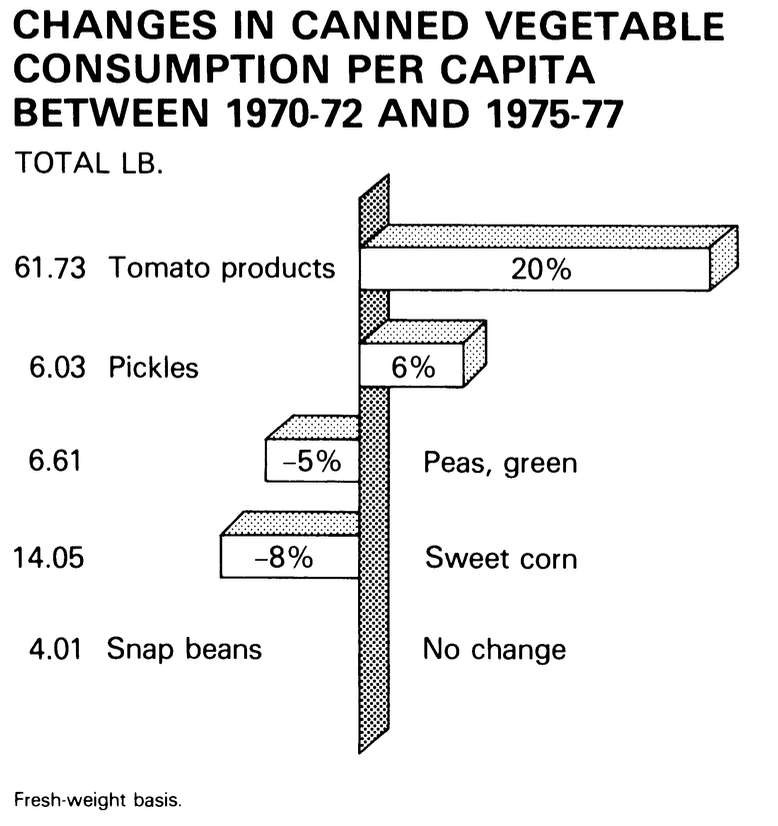
\includegraphics[width=\textwidth,height=4.16667in]{images/preferance-example2.png}

}

\subcaption{\label{fig-examp2}Figure from \emph{1978 Handbook of
Agricultural Charts. Enlargements / {[}u.s. Department of
Agriculture{]}} (1978)}

\end{minipage}%
%
\begin{minipage}{0.33\linewidth}

\centering{

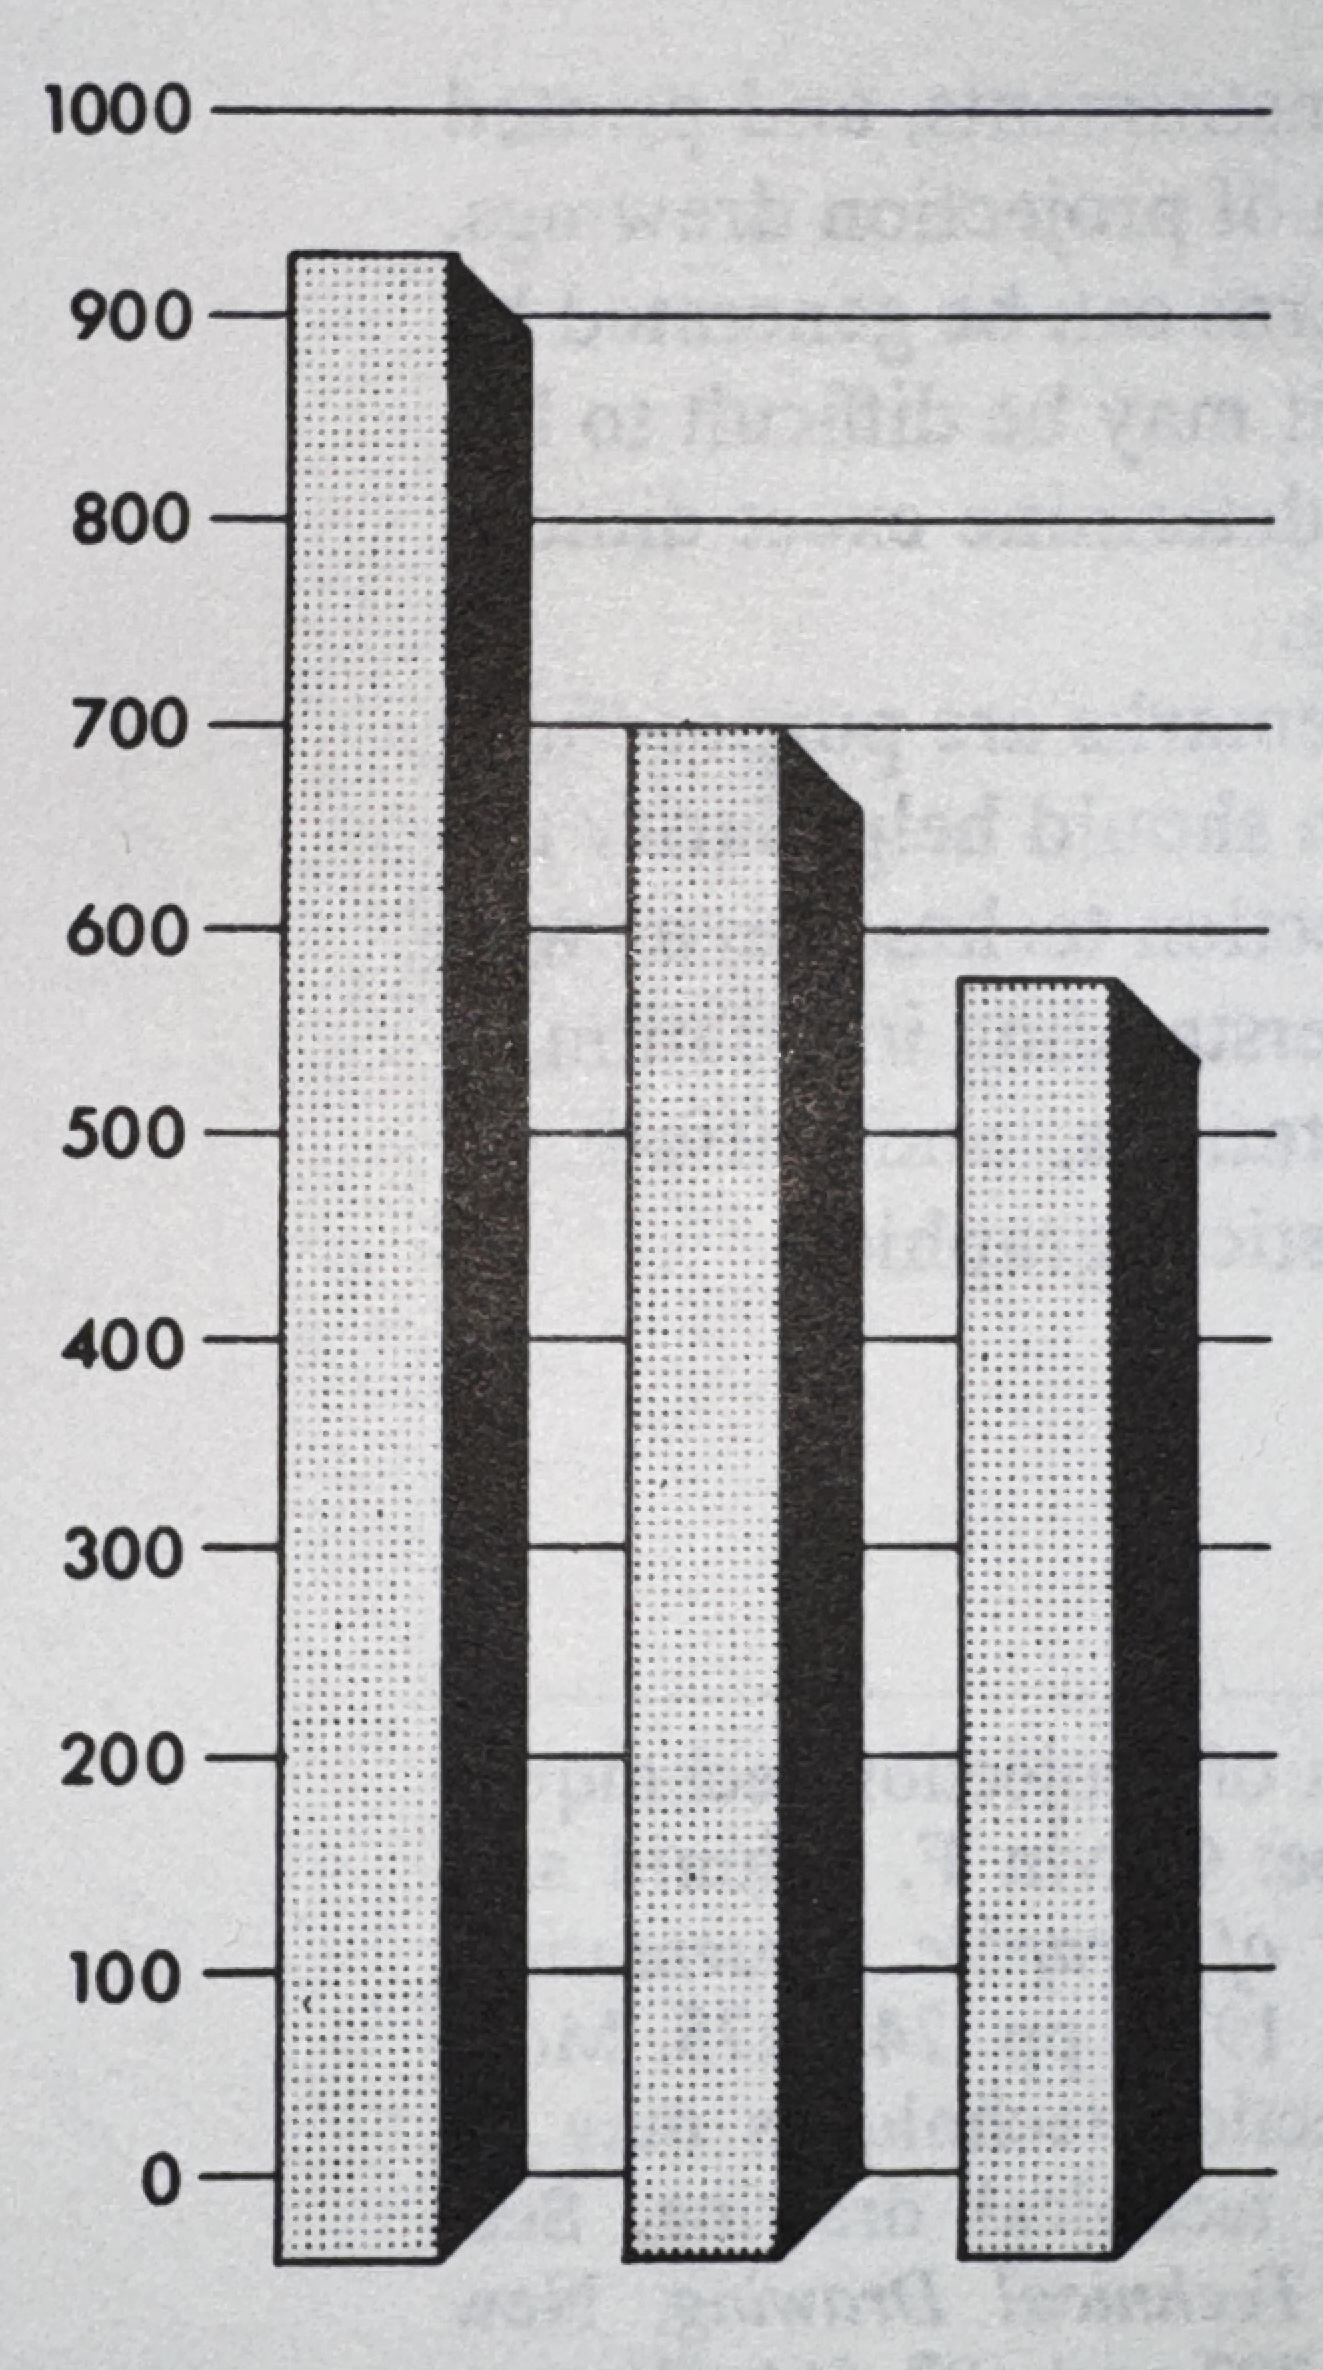
\includegraphics[width=\textwidth,height=4.16667in]{images/skewed-angle.jpg}

}

\subcaption{\label{fig-examp3}Figure from Modley (1952)}

\end{minipage}%

\caption{\label{fig-bars}Three examples of 3D bar charts found in
publications.}

\end{figure}%

\subsection{Background}\label{background-1}

The relationship between 2D and 3D bar charts presented on paper or
computer screens has been widely studied.

\begin{itemize}
\tightlist
\item
  Accuracy tends to be worse than 2D equivalents, although not always
  with statistical significance (Zacks et al. 1998; Siegrist 1996;
  Melody Carswell, Frankenberger, and Bernhard 1991; Stewart, Cipolla,
  and Best 2009).
\end{itemize}

\begin{itemize}
\tightlist
\item
  More time is needed to answer questions than 2D equivalents (Siegrist
  1996; Fischer 2000; Stewart, Cipolla, and Best 2009).
\end{itemize}

\begin{itemize}
\tightlist
\item
  2D charts chosen more often when used for numerical estimations,
  although 3D is chosen more often when presenting results to others
  (Levy et al. 1996; Fisher, Dempsey, and Marousky 1997; Stewart,
  Cipolla, and Best 2009).
\end{itemize}

\subsection{Overview of Project 1}\label{overview-of-project-1}

While early testing of statistical graphics started in the early 20th
century \footnote{Croxton and Stein (1932)} \footnote{Vanderplas, Cook,
  and Hofmann (2020)}, a major study was conducted by Cleveland and
McGill (1984) to provide guidance on better visualization practices. In
their study, numerical estimations of stimuli ratios showed differences
in various methods of data representation.

In our study, we partially replicate Cleveland and McGill's study,
including the additional factor of chart medium.

\begin{center}\rule{0.5\linewidth}{0.5pt}\end{center}

\begin{figure}

\centering{

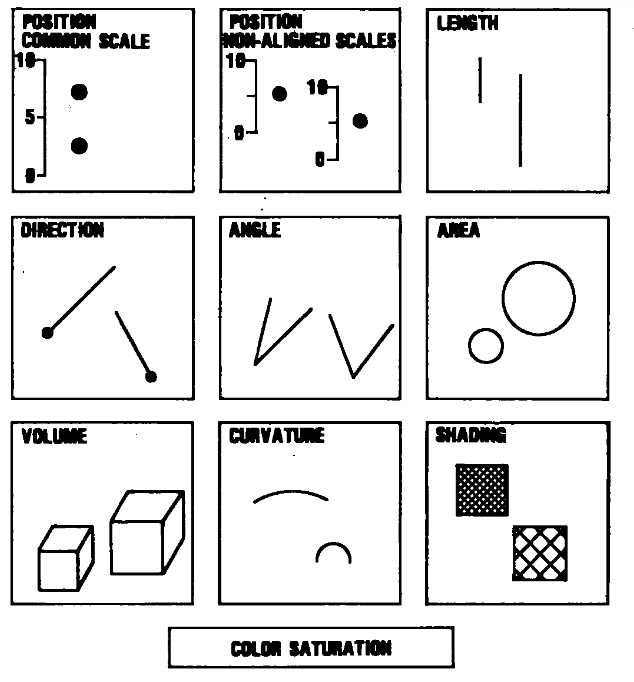
\includegraphics{images/cm-fig1.png}

}

\caption{\label{fig-cmept}Examples of EPTs listed in Figure 1 of
Cleveland and McGill (1984).}

\end{figure}%

\begin{center}\rule{0.5\linewidth}{0.5pt}\end{center}

\subsection{Cleveland and McGill (1984)}\label{cleveland1984}

\subsubsection{Stimuli}\label{stimuli}

\begin{itemize}
\tightlist
\item
  Target stimuli followed
  \(s_i=10 \times 10^{(i-1)/12},\quad i=1,\dots, 10\)
\item
  Ratios of target stimuli: 0.178, 0.261, 0.383, 0.464 (twice), 0.562,
  0.681 (twice), 0.825 (twice)
\end{itemize}

All non-target stimuli were chosen at random, subject to constraints.

\begin{Shaded}
\begin{Highlighting}[]
\NormalTok{stimuli }\OtherTok{\textless{}{-}} \DecValTok{10}\SpecialCharTok{*}\DecValTok{10}\SpecialCharTok{\^{}}\NormalTok{((}\DecValTok{1}\SpecialCharTok{:}\DecValTok{10{-}1}\NormalTok{)}\SpecialCharTok{/}\DecValTok{12}\NormalTok{)}
\FunctionTok{ggplot}\NormalTok{(}\AttributeTok{mapping =} \FunctionTok{aes}\NormalTok{(}\AttributeTok{x =} \DecValTok{1}\SpecialCharTok{:}\DecValTok{10}\NormalTok{, }\AttributeTok{y =}\NormalTok{ stimuli)) }\SpecialCharTok{+} 
  \FunctionTok{geom\_bar}\NormalTok{(}\AttributeTok{stat =} \StringTok{\textquotesingle{}identity\textquotesingle{}}\NormalTok{, }\AttributeTok{color =} \StringTok{\textquotesingle{}black\textquotesingle{}}\NormalTok{, }\AttributeTok{width =} \DecValTok{1}\NormalTok{, }\AttributeTok{fill =} \StringTok{\textquotesingle{}\#B50000\textquotesingle{}}\NormalTok{) }\SpecialCharTok{+} 
  \FunctionTok{scale\_x\_continuous}\NormalTok{(}\AttributeTok{breaks =} \DecValTok{1}\SpecialCharTok{:}\DecValTok{10}\NormalTok{) }\SpecialCharTok{+} 
  \FunctionTok{scale\_y\_continuous}\NormalTok{(}\AttributeTok{breaks =} \FunctionTok{c}\NormalTok{(}\DecValTok{0}\NormalTok{,stimuli), }\AttributeTok{labels =} \FunctionTok{round}\NormalTok{(}\FunctionTok{c}\NormalTok{(}\DecValTok{0}\NormalTok{,stimuli),}\DecValTok{1}\NormalTok{), }\AttributeTok{limits =} \FunctionTok{c}\NormalTok{(}\DecValTok{0}\NormalTok{, }\DecValTok{60}\NormalTok{),}
                     \AttributeTok{expand =} \FunctionTok{c}\NormalTok{(}\DecValTok{0}\NormalTok{,}\DecValTok{0}\NormalTok{)) }\SpecialCharTok{+}
  \FunctionTok{labs}\NormalTok{(}\AttributeTok{x =} \StringTok{\textquotesingle{}\textquotesingle{}}\NormalTok{, }\AttributeTok{y =} \StringTok{\textquotesingle{}Stimuli Value\textquotesingle{}}\NormalTok{) }\SpecialCharTok{+} 
  \FunctionTok{theme\_bw}\NormalTok{() }\SpecialCharTok{+} 
  \FunctionTok{theme}\NormalTok{(}\AttributeTok{aspect.ratio =} \DecValTok{1}\SpecialCharTok{/}\DecValTok{2}\NormalTok{, }
        \AttributeTok{panel.grid.major.x =} \FunctionTok{element\_blank}\NormalTok{(),}
        \AttributeTok{panel.grid.minor.x =} \FunctionTok{element\_blank}\NormalTok{(),}
        \AttributeTok{axis.text.x =} \FunctionTok{element\_blank}\NormalTok{(),}
        \AttributeTok{axis.text.y =} \FunctionTok{element\_text}\NormalTok{(}\AttributeTok{size =} \DecValTok{16}\NormalTok{, }\AttributeTok{angle =} \DecValTok{30}\NormalTok{, }\AttributeTok{hjust =} \DecValTok{1}\NormalTok{),}
        \AttributeTok{axis.title.y =} \FunctionTok{element\_text}\NormalTok{(}\AttributeTok{size =} \DecValTok{14}\NormalTok{),}
        \AttributeTok{axis.ticks.x =} \FunctionTok{element\_blank}\NormalTok{(),}
        \AttributeTok{panel.grid.minor =} \FunctionTok{element\_blank}\NormalTok{())}

\NormalTok{ratios }\OtherTok{\textless{}{-}} \FunctionTok{c}\NormalTok{(}\FloatTok{0.178}\NormalTok{, }\FloatTok{0.261}\NormalTok{, }\FloatTok{0.383}\NormalTok{, }\FloatTok{0.464}\NormalTok{, }\FloatTok{0.562}\NormalTok{, }\FloatTok{0.681}\NormalTok{, }\FloatTok{0.825}\NormalTok{)}
\NormalTok{twice }\OtherTok{\textless{}{-}} \FunctionTok{c}\NormalTok{(}\FloatTok{0.464}\NormalTok{, }\FloatTok{0.681}\NormalTok{, }\FloatTok{0.825}\NormalTok{)}

\FunctionTok{ggplot}\NormalTok{(}\AttributeTok{mapping =} \FunctionTok{aes}\NormalTok{(}\AttributeTok{x =} \DecValTok{1}\SpecialCharTok{:}\FunctionTok{length}\NormalTok{(ratios), }\AttributeTok{y =}\NormalTok{ ratios)) }\SpecialCharTok{+} 
  \FunctionTok{geom\_bar}\NormalTok{(}\AttributeTok{stat =} \StringTok{\textquotesingle{}identity\textquotesingle{}}\NormalTok{, }\AttributeTok{color =} \StringTok{\textquotesingle{}black\textquotesingle{}}\NormalTok{, }\AttributeTok{width =} \DecValTok{1}\NormalTok{, }\AttributeTok{fill =} \StringTok{\textquotesingle{}\#B50000\textquotesingle{}}\NormalTok{) }\SpecialCharTok{+} 
  \FunctionTok{scale\_x\_continuous}\NormalTok{(}\AttributeTok{breaks =} \DecValTok{1}\SpecialCharTok{:}\DecValTok{10}\NormalTok{) }\SpecialCharTok{+} 
  \FunctionTok{scale\_y\_continuous}\NormalTok{(}\AttributeTok{breaks =} \FunctionTok{c}\NormalTok{(}\DecValTok{0}\NormalTok{,ratios), }\AttributeTok{labels =} \FunctionTok{round}\NormalTok{(}\FunctionTok{c}\NormalTok{(}\DecValTok{0}\NormalTok{,ratios),}\DecValTok{3}\NormalTok{), }\AttributeTok{limits =} \FunctionTok{c}\NormalTok{(}\DecValTok{0}\NormalTok{, }\DecValTok{1}\NormalTok{),}
                     \AttributeTok{expand =} \FunctionTok{c}\NormalTok{(}\DecValTok{0}\NormalTok{,}\DecValTok{0}\NormalTok{)) }\SpecialCharTok{+}
  \FunctionTok{labs}\NormalTok{(}\AttributeTok{x =} \StringTok{\textquotesingle{}\textquotesingle{}}\NormalTok{, }\AttributeTok{y =} \StringTok{\textquotesingle{}Ratio\textquotesingle{}}\NormalTok{,}
       \AttributeTok{caption =} \StringTok{\textquotesingle{}* = used twice\textquotesingle{}}\NormalTok{) }\SpecialCharTok{+} 
  \FunctionTok{annotate}\NormalTok{(}\StringTok{\textquotesingle{}text\textquotesingle{}}\NormalTok{, }\AttributeTok{x =}\NormalTok{ (}\DecValTok{1}\SpecialCharTok{:}\FunctionTok{length}\NormalTok{(ratios))[ratios }\SpecialCharTok{\%in\%}\NormalTok{ twice], }\AttributeTok{y =}\NormalTok{ twice}\FloatTok{{-}0.1}\NormalTok{, }\AttributeTok{label =} \StringTok{\textquotesingle{}*\textquotesingle{}}\NormalTok{, }\AttributeTok{size =} \DecValTok{10}\NormalTok{) }\SpecialCharTok{+}
  \FunctionTok{theme\_bw}\NormalTok{() }\SpecialCharTok{+} 
  \FunctionTok{theme}\NormalTok{(}\AttributeTok{aspect.ratio =} \DecValTok{1}\SpecialCharTok{/}\DecValTok{2}\NormalTok{, }
        \AttributeTok{panel.grid.major.x =} \FunctionTok{element\_blank}\NormalTok{(),}
        \AttributeTok{panel.grid.minor.x =} \FunctionTok{element\_blank}\NormalTok{(),}
        \AttributeTok{axis.text.x =} \FunctionTok{element\_blank}\NormalTok{(),}
        \AttributeTok{axis.text.y =} \FunctionTok{element\_text}\NormalTok{(}\AttributeTok{size =} \DecValTok{16}\NormalTok{, }\AttributeTok{angle =} \DecValTok{30}\NormalTok{, }\AttributeTok{hjust =} \DecValTok{1}\NormalTok{),}
        \AttributeTok{axis.title.y =} \FunctionTok{element\_text}\NormalTok{(}\AttributeTok{size =} \DecValTok{14}\NormalTok{),}
        \AttributeTok{plot.caption =} \FunctionTok{element\_text}\NormalTok{(}\AttributeTok{size =} \DecValTok{10}\NormalTok{),}
        \AttributeTok{axis.ticks.x =} \FunctionTok{element\_blank}\NormalTok{(),}
        \AttributeTok{panel.grid.minor =} \FunctionTok{element\_blank}\NormalTok{())}
\end{Highlighting}
\end{Shaded}

\begin{figure}

\begin{minipage}{0.50\linewidth}

\centering{

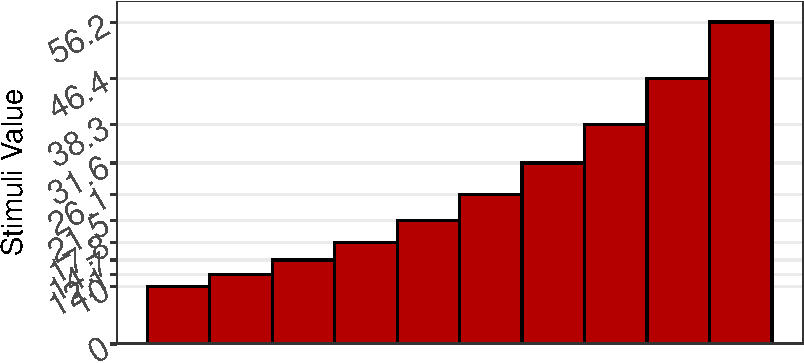
\includegraphics[width=\textwidth,height=1\textheight]{index_files/figure-pdf/fig-cm-values-1.pdf}

}

\subcaption{\label{fig-cm-values-1}Stimuli Values}

\end{minipage}%
%
\begin{minipage}{0.50\linewidth}

\centering{

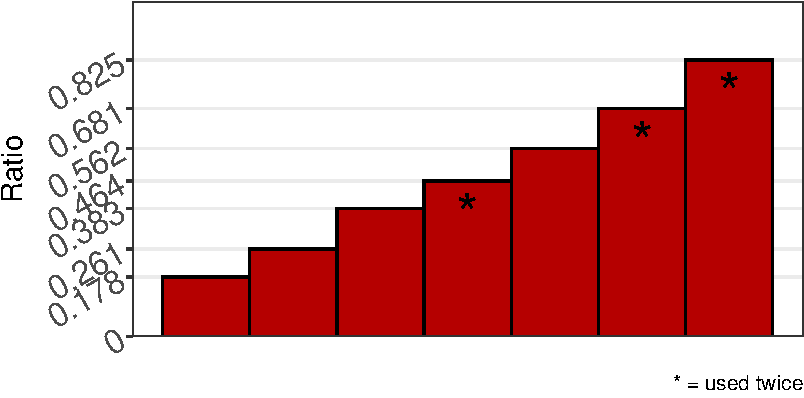
\includegraphics[width=\textwidth,height=1\textheight]{index_files/figure-pdf/fig-cm-values-2.pdf}

}

\subcaption{\label{fig-cm-values-2}Ratios}

\end{minipage}%

\caption{\label{fig-cm-values}Stimuli and ratios used by Cleveland and
McGill (1984).}

\end{figure}%

\subsection{Cleveland and McGill (1984)}\label{cleveland1984-1}

\subsubsection{Chart Types}\label{chart-types}

\begin{figure}

\centering{

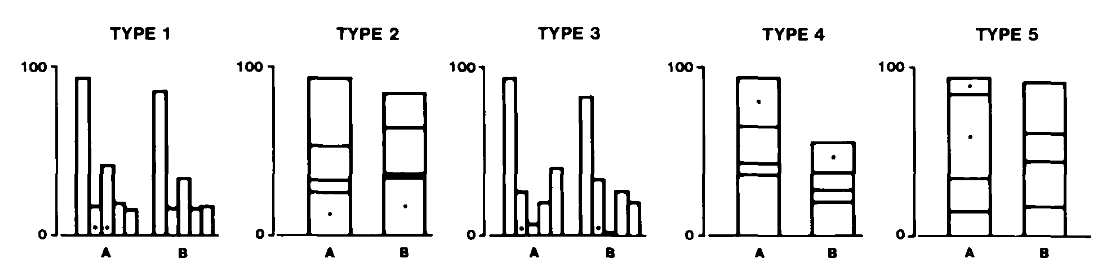
\includegraphics{images/cm-types.png}

}

\caption{\label{fig-cmtypes}Chart types used by Cleveland and McGill
(1984)}

\end{figure}%

\begin{itemize}
\tightlist
\item
  Type 1: Position along a common scale
\item
  Type 2: Position along a common scale
\item
  Type 3: Position along a common scale
\item
  Type 4: Length
\item
  Type 5: Length
\end{itemize}

\subsection{Cleveland and McGill (1984)}\label{cleveland1984-2}

\subsubsection{Experimental Design}\label{experimental-design}

\begin{itemize}
\tightlist
\item
  Treatments

  \begin{itemize}
  \tightlist
  \item
    Ratio (10)
  \item
    Graph type (5)
  \end{itemize}
\item
  Responses

  \begin{itemize}
  \tightlist
  \item
    Correctly identify smaller value of stimuli pair
  \item
    \(\log_2(|\text{Error}|+1/8)\)
  \end{itemize}
\item
  Procedure

  \begin{itemize}
  \tightlist
  \item
    5 practice graphs followed by 50 graphs in an identical randomized
    order for each participant
  \end{itemize}
\end{itemize}

\subsection{Project 1}\label{project-1}

Our first project partially replicates and expands on the first
experiment by Cleveland and McGill (1984).

\begin{Shaded}
\begin{Highlighting}[]
\FunctionTok{tribble}\NormalTok{(}
  \SpecialCharTok{\textasciitilde{}}\NormalTok{Component,   }\SpecialCharTok{\textasciitilde{}}\StringTok{\textasciigrave{}}\AttributeTok{Our Research}\StringTok{\textasciigrave{}}\NormalTok{,    }\SpecialCharTok{\textasciitilde{}}\StringTok{\textasciigrave{}}\AttributeTok{Cleveland and McGill}\StringTok{\textasciigrave{}}\NormalTok{,}
\StringTok{\textquotesingle{}\# of ratios\textquotesingle{}}\NormalTok{,  }\StringTok{\textquotesingle{}7 ratios\textquotesingle{}}\NormalTok{, }\StringTok{\textquotesingle{}10 ratios (7 unique)\textquotesingle{}}\NormalTok{,}
\StringTok{\textquotesingle{}\# of chart types\textquotesingle{}}\NormalTok{, }\StringTok{\textquotesingle{}2\textquotesingle{}}\NormalTok{,    }\StringTok{\textquotesingle{}5\textquotesingle{}}\NormalTok{,}
\StringTok{\textquotesingle{}\# of media types\textquotesingle{}}\NormalTok{, }\StringTok{\textquotesingle{}3 (2D and 3D digitized, 3D printed)\textquotesingle{}}\NormalTok{,  }\StringTok{\textquotesingle{}1 (2D on paper)\textquotesingle{}}\NormalTok{,}
\StringTok{\textquotesingle{}\# of charts/participant\textquotesingle{}}\NormalTok{, }\StringTok{\textquotesingle{}15\textquotesingle{}}\NormalTok{,    }\StringTok{\textquotesingle{}50\textquotesingle{}}
\NormalTok{) }\SpecialCharTok{\%\textgreater{}\%} 
\NormalTok{  knitr}\SpecialCharTok{::}\FunctionTok{kable}\NormalTok{()}
\end{Highlighting}
\end{Shaded}

\begin{longtable}[]{@{}
  >{\raggedright\arraybackslash}p{(\columnwidth - 4\tabcolsep) * \real{0.2963}}
  >{\raggedright\arraybackslash}p{(\columnwidth - 4\tabcolsep) * \real{0.4444}}
  >{\raggedright\arraybackslash}p{(\columnwidth - 4\tabcolsep) * \real{0.2593}}@{}}
\toprule\noalign{}
\begin{minipage}[b]{\linewidth}\raggedright
Component
\end{minipage} & \begin{minipage}[b]{\linewidth}\raggedright
Our Research
\end{minipage} & \begin{minipage}[b]{\linewidth}\raggedright
Cleveland and McGill
\end{minipage} \\
\midrule\noalign{}
\endhead
\bottomrule\noalign{}
\endlastfoot
\# of ratios & 7 ratios & 10 ratios (7 unique) \\
\# of chart types & 2 & 5 \\
\# of media types & 3 (2D and 3D digitized, 3D printed) & 1 (2D on
paper) \\
\# of charts/participant & 15 & 50 \\
\end{longtable}

To get 15 graphs per participant, we used incomplete blocking of 5 on
the seven ratios. The type of chart was randomly allotted so that number
of Type 1 and Type 3 charts were approximately the same.

After the pilot study, a static 3D chart was included into the study.

\subsection{Project 1 Chart Examples}\label{project-1-chart-examples}

\begin{figure}

\centering{

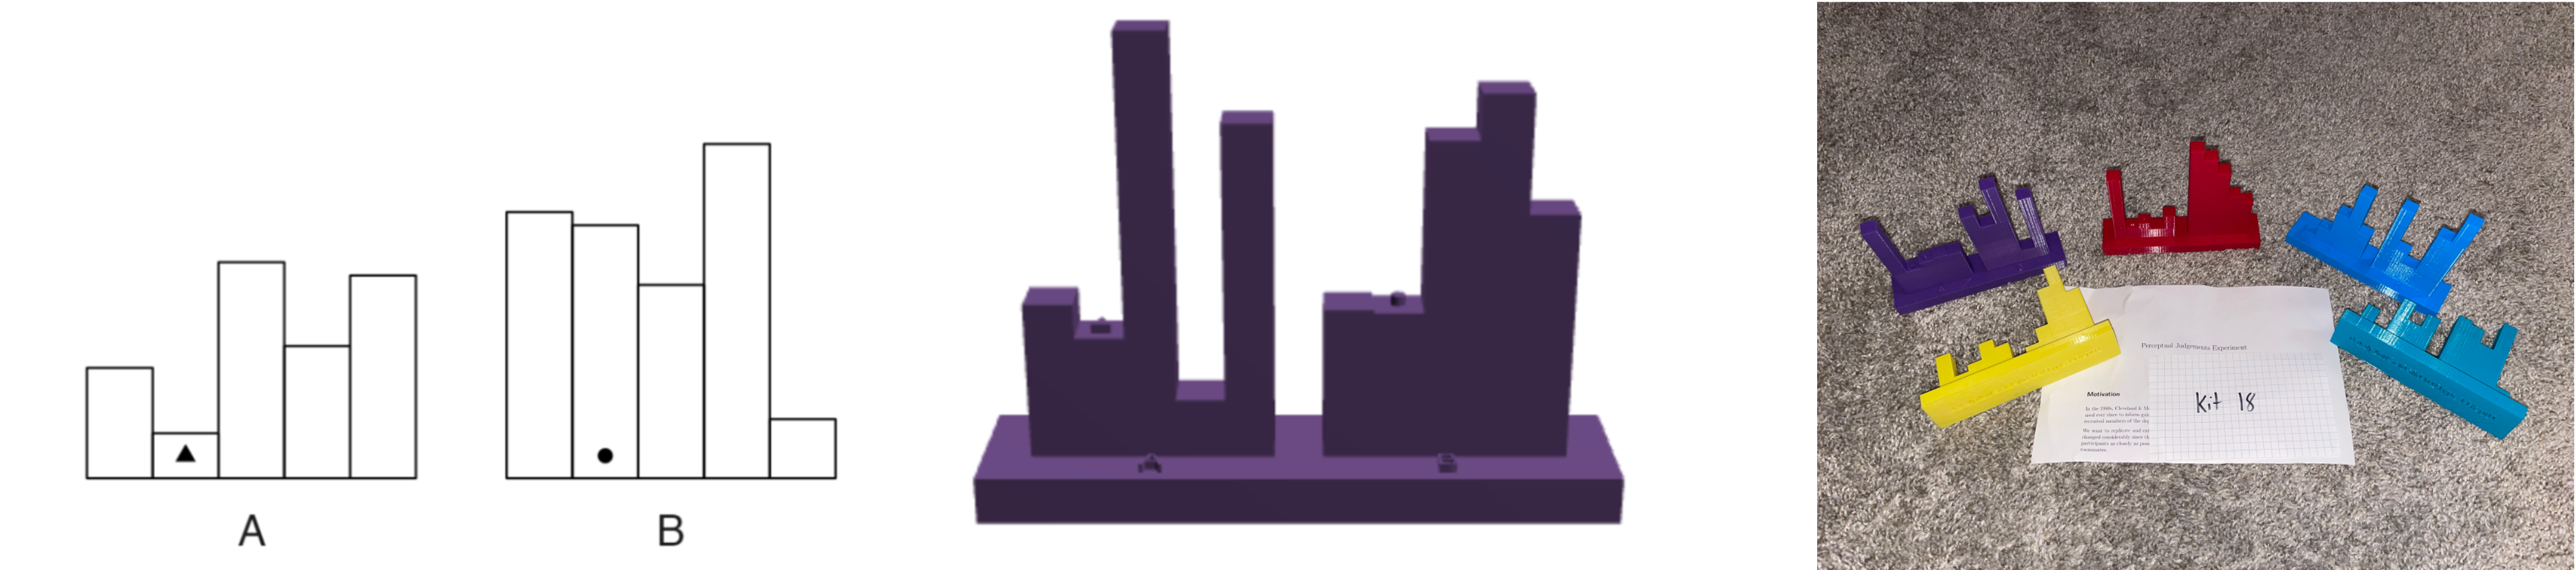
\includegraphics{images/pilot-charts.png}

}

\caption{\label{fig-p1-charts}Charts used in bar chart pilot study.}

\end{figure}%

\subsection{Project 1 Results}\label{project-1-results}

\begin{figure}

\centering{

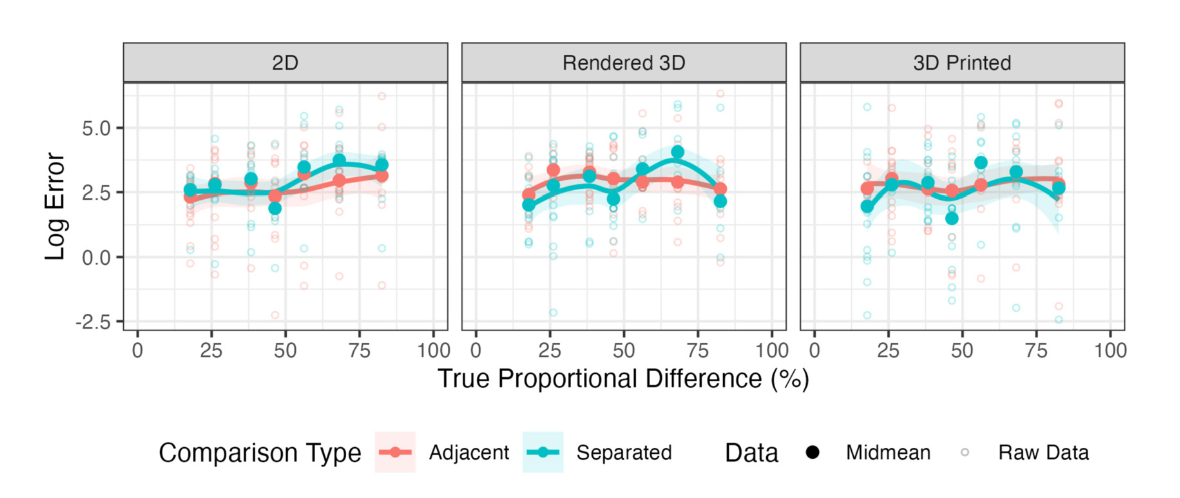
\includegraphics{images/project1-results.png}

}

\caption{\label{fig-project1-results}Results from pilot study conducted
for the 3D bar chart experiment.}

\end{figure}%

Using a generalized additive model (GAM), the only significant effect
was either replicating Type 1 or Type 3. In the pilot study, we had 38
participants, so it is likely that the experiment was under-powered.

\begin{itemize}
\tightlist
\item
  Integration of the experiment into Stat 218 has provided many more
  responses, but results have not yet been analyzed.
\end{itemize}

\section{Project 2: Experiential
Learning}\label{project-2-experiential-learning}

\subsection{Experiential Learning}\label{experiential-learning}

In a dual purpose role, a large sample was obtained for the two previous
projects by incorporating the experiments as an experiential learning
opportunity for Stat 218 students. This is a six stage project that
follows students from participants to consumers of scientific knowledge.

\textbf{Informed Consent}

\begin{itemize}
\tightlist
\item
  Obtain consent
\item
  Confirm age of majority (≥19)
\end{itemize}

\textbf{Pre-experiment}

\begin{itemize}
\tightlist
\item
  How does the scientific process differ between researchers and the
  general population
\end{itemize}

\textbf{Experiment}

\begin{itemize}
\tightlist
\item
  Provide completion code to show proof of experiment participation
\end{itemize}

\subsection{Experiential Learning}\label{experiential-learning-1}

\textbf{Post Experiment}

\begin{itemize}
\tightlist
\item
  What was the purpose of experiment?
\item
  What were the hypotheses?
\item
  What are the sources of error?
\item
  What were the variables?
\item
  What elements of experimental design were present?
\end{itemize}

\textbf{Abstract}

\begin{itemize}
\tightlist
\item
  What components of the experiment are now clearer?
\end{itemize}

\textbf{Presentation}

\begin{itemize}
\tightlist
\item
  How did the information you gained from each stage differ?
\item
  What was emphasized in the presentation that wasn't emphasized in the
  the abstract?
\item
  What critiques do you have of the study?
\item
  Did you prefer the abstract or presentation?
\end{itemize}

\begin{center}\rule{0.5\linewidth}{0.5pt}\end{center}

\begin{figure}

\centering{

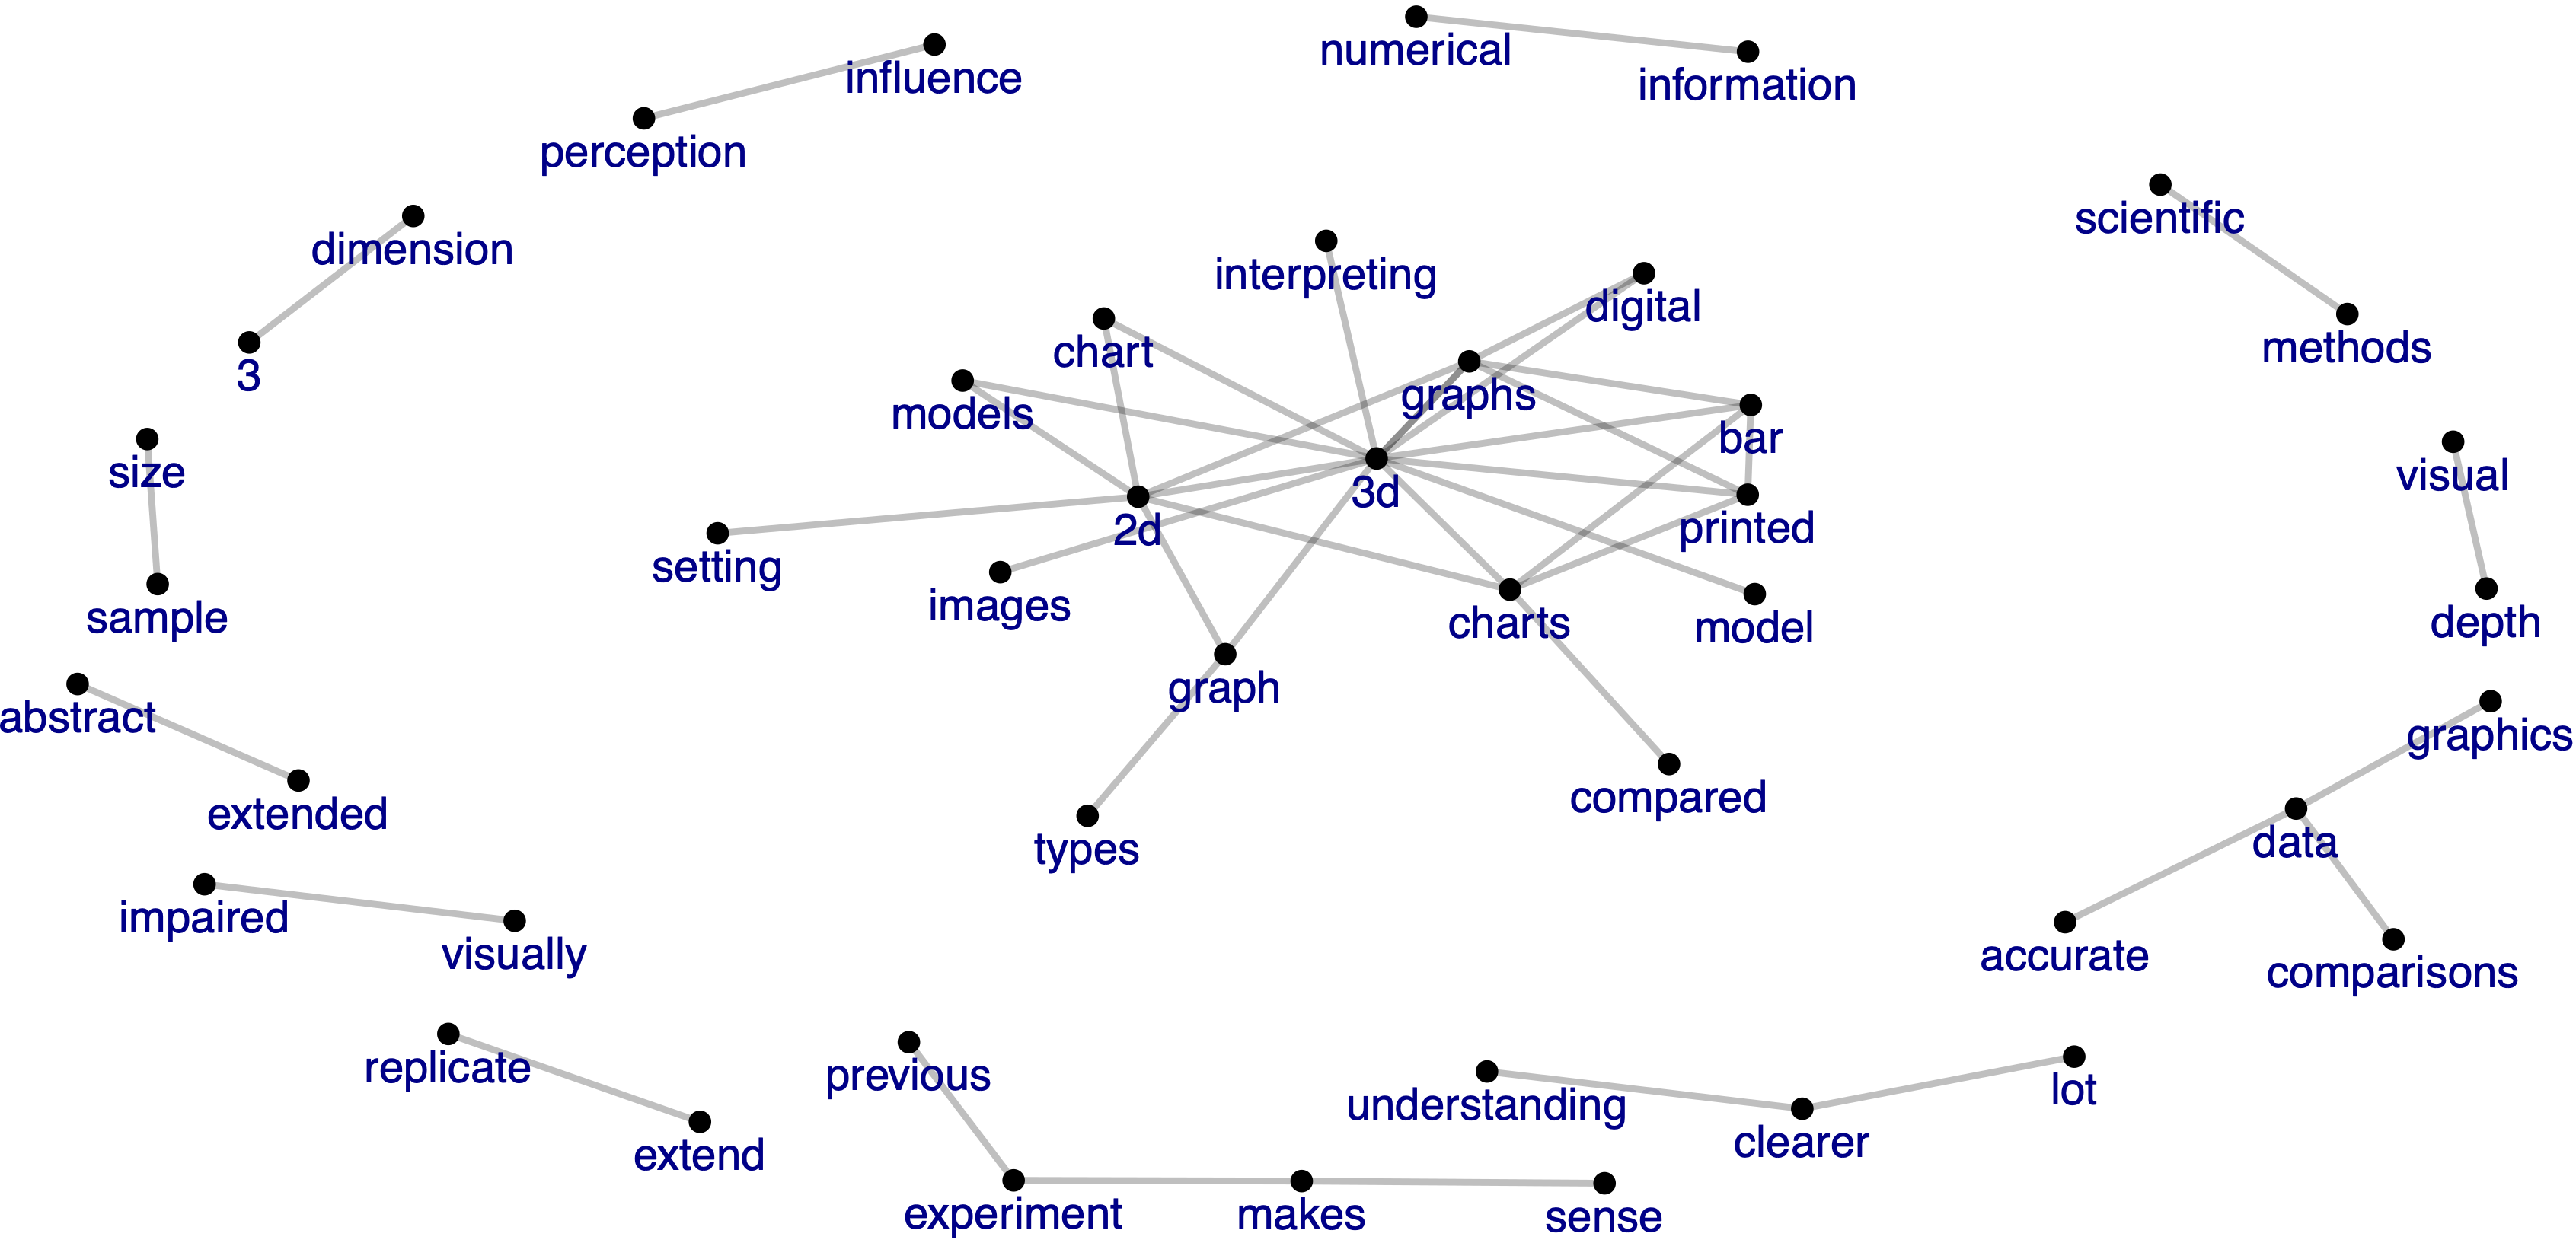
\includegraphics{images/bigram-abstract.png}

}

\caption{\label{fig-bigram}Word bigram from the abstract reflection
module. Students answered the question: ``What components of the
experiment are clearer now than they were as a participant? What
questions do you still have for the experimenter? Write 3-5 sentences
reflecting on the abstract.''}

\end{figure}%

\section{Project 3: 3D Heat Maps}\label{project-3-3d-heat-maps}

\subsection{3D Heat Maps}\label{d-heat-maps}

\begin{figure}

\begin{minipage}{0.50\linewidth}

\centering{

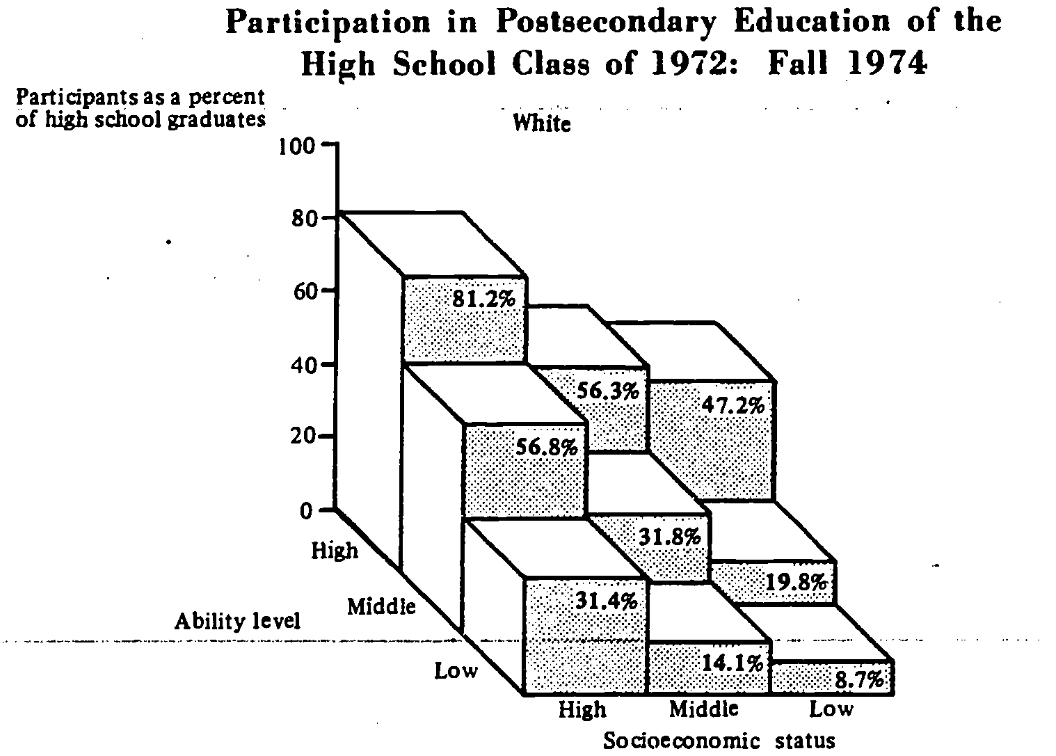
\includegraphics[width=\textwidth,height=4.16667in]{images/heatmap3d.png}

}

\subcaption{\label{fig-nat77}Figure from for Educational Statistics et
al. (1977)}

\end{minipage}%
%
\begin{minipage}{0.50\linewidth}

\centering{

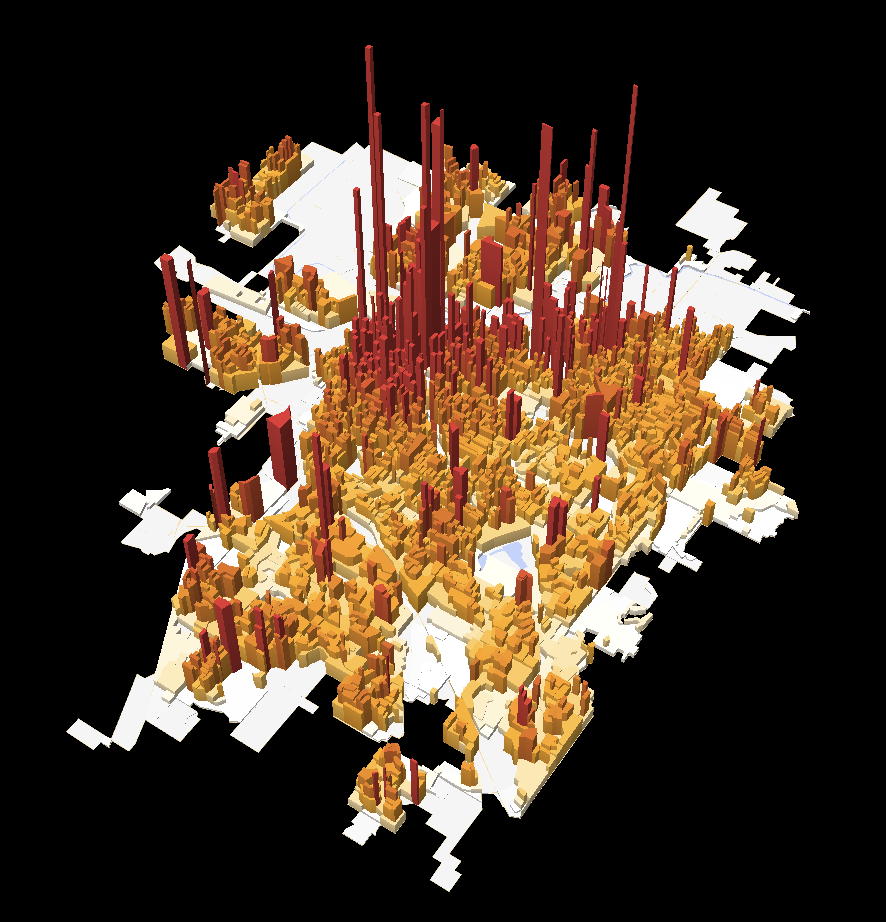
\includegraphics[width=\textwidth,height=4.16667in]{images/lincoln-pop.png}

}

\subcaption{\label{fig-lincoln-pop}Figure from {``{3D Population
Density} of the {US} - {HomeArea}.com''} (n.d.)}

\end{minipage}%

\caption{\label{fig-heatmaps}Examples of 3D heat maps.}

\end{figure}%

\subsection{Background}\label{background-2}

Unlike decorative 3D elements, direct comparisons of dimensionality is
more limited when the third dimension coveys information.

\begin{itemize}
\tightlist
\item
  Accuracy is worse for volumes than for areas (Croxton and Stein 1932).
\end{itemize}

\begin{itemize}
\tightlist
\item
  3D charts can sometimes better encode information than 2D charts
  (Barfield and Robless 1989).
\end{itemize}

\begin{itemize}
\tightlist
\item
  3D heat maps have lower error rates than 2D heat maps in virtual
  reality (Kraus et al. 2020).
\end{itemize}

\begin{itemize}
\tightlist
\item
  Kraus et al. (2020) talks about more time needed for 3D charts
\item
  Also, Kraus et al. (2020) mentioned 2D was better for overview tasks
\end{itemize}

\subsection{Overview of Project 3}\label{overview-of-project-3}

We maintain the same objective when adding information to the third
dimension: does numerical accuracy of ratio estimations differ between
dimensionality and projections of chart types. However, it is important
to note that direct translations of 2D and 3D heatmaps require different
visual cues.

\begin{figure}

\begin{minipage}{0.50\linewidth}

\centering{

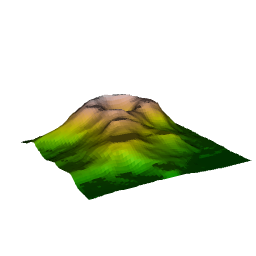
\includegraphics{images/height-color-0.3.png}

}

\subcaption{\label{fig-flat3d}Flatter height scale}

\end{minipage}%
%
\begin{minipage}{0.50\linewidth}

\centering{

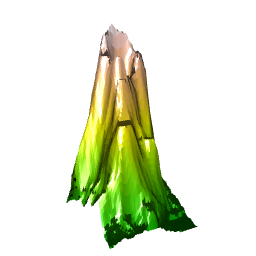
\includegraphics{images/height-color-2.png}

}

\subcaption{\label{fig-tall3d}Stretched height scale}

\end{minipage}%

\caption{\label{fig-color-height}Two figures representing the volcano
dataset (R Core Team 2024) using different height scaling factors. Both
figures use the same color scale, but there is no ``correct''
translation of color into the measurable height.}

\end{figure}%

2D heat maps use color, 3D heat maps use height and can possibly use
color as well.

\subsection{Stimuli Construction}\label{stimuli-construction}

\begin{Shaded}
\begin{Highlighting}[]
\FunctionTok{load}\NormalTok{(}\StringTok{\textquotesingle{}stimuli.rda\textquotesingle{}}\NormalTok{)}
\end{Highlighting}
\end{Shaded}

The design of the 3D heat map experiment uses the method of constant
stimuli: ratios are estimated with respect to one stimuli height that
remains the same.

Setting 50 as the constant and 90 as the maximum, a sequence of stimuli
are chosen by equally partitioning the ratios between \(50/50=1\) and
\(50/90\approx0.556\). The same ratios are used when setting 50 as the
maximum in the stimuli pair.

\begin{Shaded}
\begin{Highlighting}[]
\NormalTok{stimuli }\SpecialCharTok{\%\textgreater{}\%} 
  \FunctionTok{ggplot}\NormalTok{(}\AttributeTok{mapping =} \FunctionTok{aes}\NormalTok{(}\AttributeTok{x =}\NormalTok{ pair\_id, }\AttributeTok{y =}\NormalTok{ values)) }\SpecialCharTok{+} 
  \FunctionTok{geom\_bar}\NormalTok{(}\AttributeTok{stat =} \StringTok{\textquotesingle{}identity\textquotesingle{}}\NormalTok{, }\AttributeTok{width =} \DecValTok{1}\NormalTok{, }\AttributeTok{color =} \StringTok{\textquotesingle{}black\textquotesingle{}}\NormalTok{, }\AttributeTok{fill =} \StringTok{\textquotesingle{}\#B50000\textquotesingle{}}\NormalTok{) }\SpecialCharTok{+} 
  \FunctionTok{geom\_text}\NormalTok{(}\FunctionTok{aes}\NormalTok{(}\AttributeTok{label =} \FunctionTok{round}\NormalTok{(values, }\DecValTok{1}\NormalTok{), }\AttributeTok{y =} \DecValTok{5}\NormalTok{), }\AttributeTok{size =} \DecValTok{7}\NormalTok{) }\SpecialCharTok{+} 
  \FunctionTok{theme\_minimal}\NormalTok{() }\SpecialCharTok{+} 
  \FunctionTok{annotate}\NormalTok{(}\StringTok{\textquotesingle{}text\textquotesingle{}}\NormalTok{, }\AttributeTok{x =} \DecValTok{5}\NormalTok{, }\AttributeTok{y =} \DecValTok{25}\NormalTok{, }\AttributeTok{label =} \StringTok{\textquotesingle{}*\textquotesingle{}}\NormalTok{, }\AttributeTok{size =} \DecValTok{12}\NormalTok{) }\SpecialCharTok{+}
  \FunctionTok{labs}\NormalTok{(}\AttributeTok{x =} \StringTok{\textquotesingle{}\textquotesingle{}}\NormalTok{, }\AttributeTok{y =} \StringTok{\textquotesingle{}Magnitude of Stimuli\textquotesingle{}}\NormalTok{) }\SpecialCharTok{+}
  \FunctionTok{scale\_x\_continuous}\NormalTok{(}\AttributeTok{breaks =} \DecValTok{1}\SpecialCharTok{:}\DecValTok{9}\NormalTok{) }\SpecialCharTok{+} 
  \FunctionTok{scale\_y\_continuous}\NormalTok{(}\AttributeTok{limits =} \FunctionTok{c}\NormalTok{(}\DecValTok{0}\NormalTok{, }\DecValTok{100}\NormalTok{)) }\SpecialCharTok{+}
  \FunctionTok{theme}\NormalTok{(}\AttributeTok{panel.grid.major.x =} \FunctionTok{element\_blank}\NormalTok{(),}
        \AttributeTok{panel.grid.minor.x =} \FunctionTok{element\_blank}\NormalTok{(),}
        \AttributeTok{aspect.ratio =} \DecValTok{1}\SpecialCharTok{/}\DecValTok{2}\NormalTok{,}
        \AttributeTok{axis.text.y =} \FunctionTok{element\_text}\NormalTok{(}\AttributeTok{size =} \DecValTok{12}\NormalTok{),}
        \AttributeTok{axis.title.y =} \FunctionTok{element\_text}\NormalTok{(}\AttributeTok{size =} \DecValTok{14}\NormalTok{),}
        \AttributeTok{axis.text.x =} \FunctionTok{element\_blank}\NormalTok{(),}
        \AttributeTok{panel.grid.major.y =} \FunctionTok{element\_line}\NormalTok{(}\AttributeTok{color =} \StringTok{\textquotesingle{}grey70\textquotesingle{}}\NormalTok{),}
        \AttributeTok{panel.grid.minor.y =} \FunctionTok{element\_line}\NormalTok{(}\AttributeTok{color =} \StringTok{\textquotesingle{}grey80\textquotesingle{}}\NormalTok{, }\AttributeTok{linetype =} \StringTok{\textquotesingle{}dashed\textquotesingle{}}\NormalTok{))}

\NormalTok{stimuli }\SpecialCharTok{\%\textgreater{}\%} 
  \FunctionTok{mutate}\NormalTok{(}\AttributeTok{ratio =} \FunctionTok{round}\NormalTok{(}\FunctionTok{map2\_dbl}\NormalTok{(values, constant, \textbackslash{}(x,y)(}\FunctionTok{min}\NormalTok{(x,y)}\SpecialCharTok{/}\FunctionTok{max}\NormalTok{(x,y))), }\DecValTok{2}\NormalTok{)) }\SpecialCharTok{\%\textgreater{}\%} 
  \FunctionTok{select}\NormalTok{(ratio) }\SpecialCharTok{\%\textgreater{}\%} 
  \FunctionTok{distinct}\NormalTok{() }\SpecialCharTok{\%\textgreater{}\%} 
  \FunctionTok{ggplot}\NormalTok{(}\AttributeTok{mapping =} \FunctionTok{aes}\NormalTok{(}\AttributeTok{x =} \DecValTok{1}\SpecialCharTok{:}\DecValTok{5}\NormalTok{, }\AttributeTok{y =}\NormalTok{ ratio)) }\SpecialCharTok{+} 
  \FunctionTok{geom\_bar}\NormalTok{(}\AttributeTok{stat =} \StringTok{\textquotesingle{}identity\textquotesingle{}}\NormalTok{, }\AttributeTok{width =} \DecValTok{1}\NormalTok{, }\AttributeTok{color =} \StringTok{\textquotesingle{}black\textquotesingle{}}\NormalTok{, }\AttributeTok{fill =} \StringTok{\textquotesingle{}\#B50000\textquotesingle{}}\NormalTok{) }\SpecialCharTok{+} 
  \FunctionTok{geom\_text}\NormalTok{(}\FunctionTok{aes}\NormalTok{(}\AttributeTok{label =} \FunctionTok{round}\NormalTok{(ratio, }\DecValTok{2}\NormalTok{), }\AttributeTok{y =} \FloatTok{0.125}\SpecialCharTok{/}\DecValTok{2}\NormalTok{), }\AttributeTok{size =} \DecValTok{7}\NormalTok{) }\SpecialCharTok{+} 
  \FunctionTok{annotate}\NormalTok{(}\StringTok{\textquotesingle{}text\textquotesingle{}}\NormalTok{, }\AttributeTok{x =} \DecValTok{5}\NormalTok{, }\AttributeTok{y =} \FloatTok{0.5}\NormalTok{, }\AttributeTok{label =} \StringTok{\textquotesingle{}*\textquotesingle{}}\NormalTok{, }\AttributeTok{size =} \DecValTok{12}\NormalTok{) }\SpecialCharTok{+}
  \FunctionTok{theme\_minimal}\NormalTok{() }\SpecialCharTok{+} 
  \FunctionTok{labs}\NormalTok{(}\AttributeTok{x =} \StringTok{\textquotesingle{}\textquotesingle{}}\NormalTok{, }\AttributeTok{y =} \StringTok{\textquotesingle{}Ratio of Stimuli\textquotesingle{}}\NormalTok{) }\SpecialCharTok{+}
  \FunctionTok{scale\_x\_continuous}\NormalTok{(}\AttributeTok{breaks =} \DecValTok{1}\SpecialCharTok{:}\DecValTok{5}\NormalTok{) }\SpecialCharTok{+} 
  \FunctionTok{scale\_y\_continuous}\NormalTok{(}\AttributeTok{limits =} \FunctionTok{c}\NormalTok{(}\DecValTok{0}\NormalTok{, }\DecValTok{1}\NormalTok{)) }\SpecialCharTok{+}
  \FunctionTok{theme}\NormalTok{(}\AttributeTok{panel.grid.major.x =} \FunctionTok{element\_blank}\NormalTok{(),}
        \AttributeTok{panel.grid.minor.x =} \FunctionTok{element\_blank}\NormalTok{(),}
        \AttributeTok{axis.text.x =} \FunctionTok{element\_blank}\NormalTok{(),}
        \AttributeTok{axis.text.y =} \FunctionTok{element\_text}\NormalTok{(}\AttributeTok{size =} \DecValTok{12}\NormalTok{),}
        \AttributeTok{axis.title.y =} \FunctionTok{element\_text}\NormalTok{(}\AttributeTok{size =} \DecValTok{14}\NormalTok{),}
        \AttributeTok{aspect.ratio =} \DecValTok{1}\SpecialCharTok{/}\DecValTok{2}\NormalTok{,}
        \AttributeTok{panel.grid.major.y =} \FunctionTok{element\_line}\NormalTok{(}\AttributeTok{color =} \StringTok{\textquotesingle{}grey70\textquotesingle{}}\NormalTok{),}
        \AttributeTok{panel.grid.minor.y =} \FunctionTok{element\_line}\NormalTok{(}\AttributeTok{color =} \StringTok{\textquotesingle{}grey80\textquotesingle{}}\NormalTok{, }\AttributeTok{linetype =} \StringTok{\textquotesingle{}dashed\textquotesingle{}}\NormalTok{))}
\end{Highlighting}
\end{Shaded}

\begin{figure}

\begin{minipage}{0.50\linewidth}

\centering{

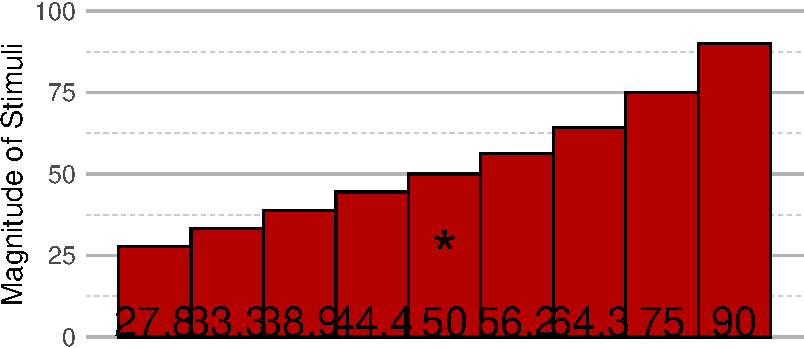
\includegraphics{index_files/figure-pdf/fig-p3-stimuli-1.pdf}

}

\subcaption{\label{fig-p3-stimuli-1}Stimuli values}

\end{minipage}%
%
\begin{minipage}{0.50\linewidth}

\centering{

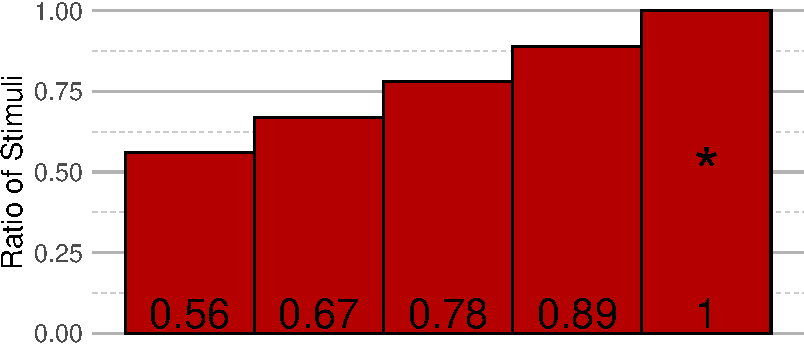
\includegraphics{index_files/figure-pdf/fig-p3-stimuli-2.pdf}

}

\subcaption{\label{fig-p3-stimuli-2}Ratios of stimuli pairs}

\end{minipage}%

\caption{\label{fig-p3-stimuli}Stimuli used in 3D heat map experiment.
All values are paired with the stimuli magnitude of 50.}

\end{figure}%

\subsection{Media Types}\label{media-types}

\begin{figure}

\begin{minipage}{0.33\linewidth}

\centering{

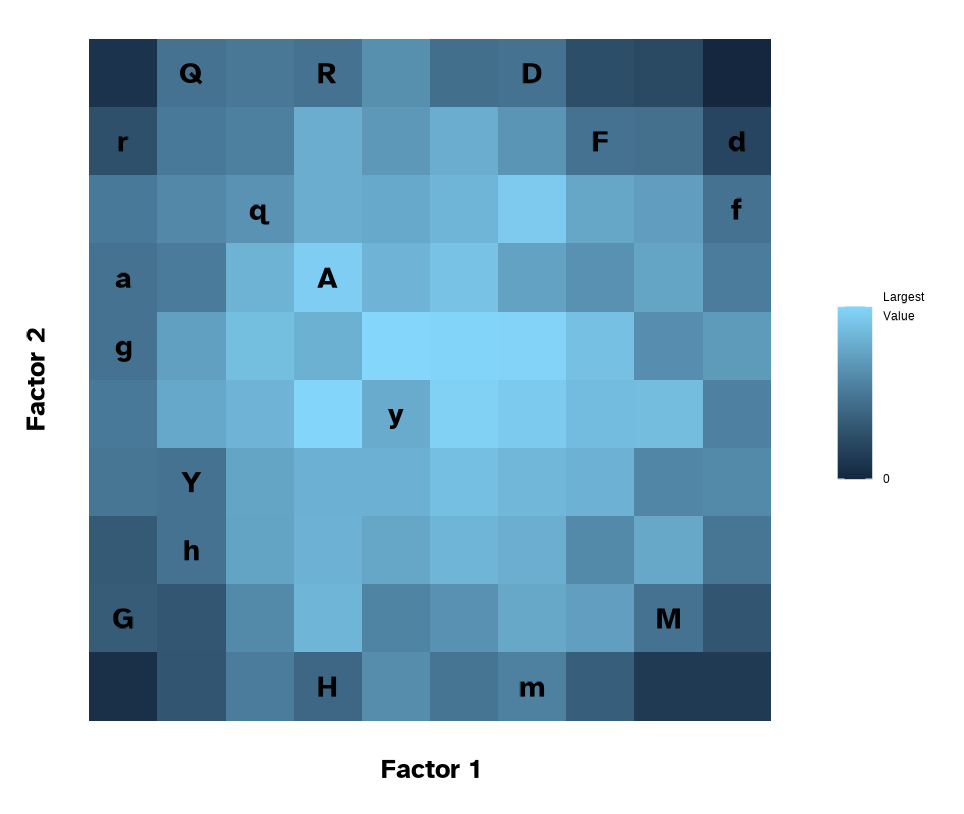
\includegraphics[width=\textwidth,height=3.125in]{images/examp2dd.png}

}

\subcaption{\label{fig-2dd}2D heatmap}

\end{minipage}%
%
\begin{minipage}{0.33\linewidth}

\centering{

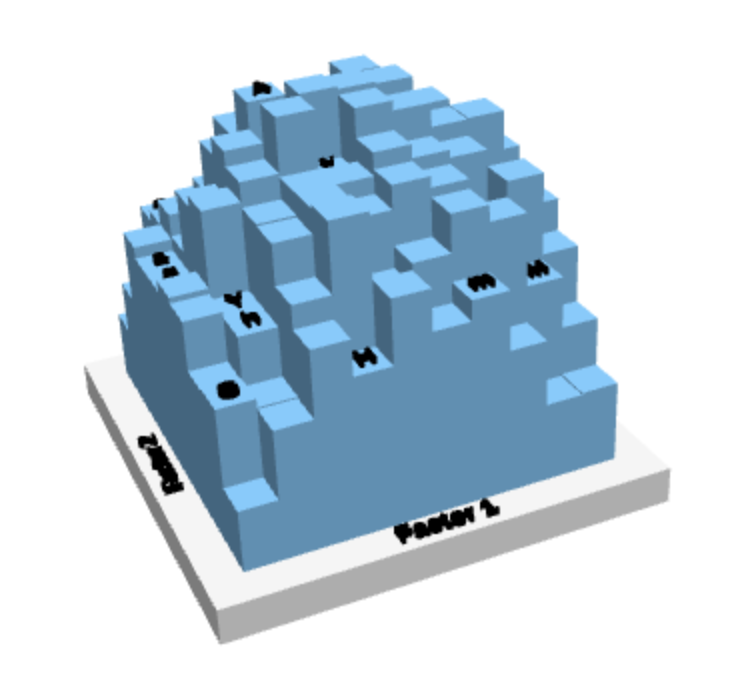
\includegraphics[width=\textwidth,height=3.125in]{images/examp3dd.png}

}

\subcaption{\label{fig-3dd}3D Digital heatmap}

\end{minipage}%
%
\begin{minipage}{0.33\linewidth}

\centering{

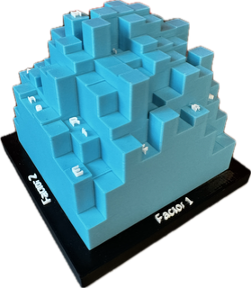
\includegraphics[width=\textwidth,height=3.125in]{images/examp3dp.png}

}

\subcaption{\label{fig-3dp}3D-Printed heatmap}

\end{minipage}%

\caption{\label{fig-heat3dexamples}Media types using dataset 1 in the 3D
heatmap experiment.}

\end{figure}%

\subsection{Procedure}\label{procedure}

\textbf{Treatment Design}

\begin{itemize}
\tightlist
\item
  9 stimuli pairs
\item
  3 media types
\item
  2 heat map datasets
\end{itemize}

\textbf{Experiment Design}

\begin{enumerate}
\def\labelenumi{\arabic{enumi}.}
\tightlist
\item
  Create incomplete blocks on stimuli pairs (choose 4 from 9)
\item
  Randomly assign participant to block on experiment initialization
\item
  Present media type x dataset in randomized order (whole-plot)
\item
  Present stimuli pair in randomized order (split-plot)
\end{enumerate}

\section{Contribution to literature}\label{contribution-to-literature}

\subsection{Contribution to
literature}\label{contribution-to-literature-1}

Nearly all studies involving statistical graphics use paper-printed or
digitized charts, resulting in a knowledge gap in statistical graphics
presented in tangible formats. Our contributions are as follows:

\begin{enumerate}
\def\labelenumi{\arabic{enumi}.}
\tightlist
\item
  Explore the relationship of physical dimensionality on bar charts /
  heat maps using numerical accuracy of ratio estimations.
\item
  Provide recommendations on the construction of 3D-printed statistical
  graphics.
\item
  Explore how students interact with the process of scientific
  investigation using a ``hands-on'' statistical study.
\end{enumerate}

Exceptions include tactile charts, virtual reality, and artistic data
physicalization. However, the interaction with these differs vastly with
our 3D printed charts.

\section{Questions?}\label{questions}

\subsection{References}\label{references}

\phantomsection\label{refs}
\begin{CSLReferences}{1}{0}
\bibitem[\citeproctext]{ref-cdi_hathitrust_hathifiles_uva_x030492864}
\emph{1978 Handbook of Agricultural Charts. Enlargements / {[}u.s.
Department of Agriculture{]}}. 1978. District of Columbia: United
States. Department of Agriculture; U.S. Dept. of Agriculture ;
Distributed by Science; Education Administration.

\bibitem[\citeproctext]{ref-3DPopulationDensity}
{``{3D Population Density} of the {US} - {HomeArea}.com.''} n.d.
https://www.homearea.com/featured/3d-population-density/\#3128000.
Accessed September 17, 2025.

\bibitem[\citeproctext]{ref-helen2016}
Armstrong, Helen. 2016. \emph{Digital Design Theory : Readings from the
Field}. Design Briefs. New York, New York: Princeton Architectural
Press.

\bibitem[\citeproctext]{ref-barfield1989}
Barfield, Woodrow, and Robert Robless. 1989. {``The Effects of Two- or
Three-Dimensional Graphics on the Problem-Solving Performance of
Experienced and Novice Decision Makers.''} \emph{Behaviour \&
Information Technology} 8 (5): 369--85.
\url{https://doi.org/10.1080/01449298908914567}.

\bibitem[\citeproctext]{ref-buja2009}
Buja, Andreas, Dianne Cook, Heike Hofmann, Michael Lawrence, Eun-Kyung
Lee, Deborah F. Swayne, and Hadley Wlckham. 2009. {``Statistical
Inference for Exploratory Data Analysis and Model Diagnostics.''}
\emph{Philosophical Transactions: Mathematical, Physical and Engineering
Sciences} 367 (1906): 4361--83.
\url{https://www.jstor.org/stable/40485732}.

\bibitem[\citeproctext]{ref-cleveland1984}
Cleveland, William S., and Robert McGill. 1984. {``Graphical Perception:
Theory, Experimentation, and Application to the Development of Graphical
Methods.''} \emph{Journal of the American Statistical Association} 79
(387): 531--54. \url{https://doi.org/10.1080/01621459.1984.10478080}.

\bibitem[\citeproctext]{ref-croxton1932}
Croxton, Frederick E., and Harold Stein. 1932. {``Graphic Comparisons by
Bars, Squares, Circles, and Cubes.''} \emph{Journal of the American
Statistical Association} 27 (177): 54--60.
\url{https://doi.org/10.1080/01621459.1932.10503227}.

\bibitem[\citeproctext]{ref-fischer2000}
Fischer, Martin H. 2000. {``Do Irrelevant Depth Cues Affect the
Comprehension of Bar Graphs?''} \emph{Applied Cognitive Psychology} 14
(2): 151--62.
\url{https://doi.org/10.1002/(SICI)1099-0720(200003/04)14:2\%3C151::AID-ACP629\%3E3.0.CO;2-Z}.

\bibitem[\citeproctext]{ref-fisher1997}
Fisher, Samuel H., John V. Dempsey, and Robert T. Marousky. 1997.
{``Data Visualization: Preference and Use of Two-Dimensional and
Three-Dimensional Graphs.''} \emph{Social Science Computer Review} 15
(3): 256--63. \url{https://doi.org/10.1177/089443939701500303}.

\bibitem[\citeproctext]{ref-national1977condition}
for Educational Statistics, National Center, National Center for
Education Statistics, United States. Office of Educational Research,
Improvement. Center for Education Statistics, and Institute of Education
Sciences (U.S.). 1977. \emph{The Condition of Education}. 1975-1979:
{DHEW} Publication. {U.S. Department of Education, Office of Educational
Research and Improvement, National Center for Education Statistics}.

\bibitem[\citeproctext]{ref-penguins}
Horst, Allison Marie, Alison Presmanes Hill, and Kristen B Gorman. 2020.
\emph{Palmerpenguins: Palmer Archipelago (Antarctica) Penguin Data}.
\url{https://doi.org/10.5281/zenodo.3960218}.

\bibitem[\citeproctext]{ref-kraus2020}
Kraus, Matthias, Katrin Angerbauer, Juri Buchmüller, Daniel Schweitzer,
Daniel A. Keim, Michael Sedlmair, and Johannes Fuchs. 2020. {``CHI '20:
CHI Conference on Human Factors in Computing Systems.''} In, 1--14.
Honolulu HI USA: ACM. \url{https://doi.org/10.1145/3313831.3376675}.

\bibitem[\citeproctext]{ref-levy1996}
Levy, Ellen, Jeff Zacks, Barbara Tversky, and Diane Schiano. 1996.
{``The SIGCHI Conference.''} In, 42--49. Vancouver, British Columbia,
Canada: ACM Press. \url{https://doi.org/10.1145/238386.238400}.

\bibitem[\citeproctext]{ref-melodycarswell1991}
Melody Carswell, C., Sylvia Frankenberger, and Donald Bernhard. 1991.
{``Graphing in Depth: Perspectives on the Use of Three-Dimensional
Graphs to Represent Lower-Dimensional Data.''} \emph{Behaviour \&
Information Technology} 10 (6): 459--74.
\url{https://doi.org/10.1080/01449299108924304}.

\bibitem[\citeproctext]{ref-ModleyRudolf1952Pag}
Modley, Rudolf. 1952. \emph{Pictographs and Graphs : How to Make and Use
Them}. New York: Harper.

\bibitem[\citeproctext]{ref-rgl}
Murdoch, Duncan, and Daniel Adler. 2024. \emph{Rgl: 3D Visualization
Using OpenGL}. \url{https://CRAN.R-project.org/package=rgl}.

\bibitem[\citeproctext]{ref-peuxf1a2020}
Peña, Alyssa, Eric Ragan, and Lane Harrison. 2020. {``Memorability of
Enhanced Informational Graphics.''} \emph{Interdisciplinary Journal of
Signage and Wayfinding} 4 (1).
\url{https://doi.org/10.15763/issn.2470-9670.2020.v4.i1.a54}.

\bibitem[\citeproctext]{ref-volcano}
R Core Team. 2024. \emph{R: A Language and Environment for Statistical
Computing}. Vienna, Austria: R Foundation for Statistical Computing.
\url{https://www.R-project.org/}.

\bibitem[\citeproctext]{ref-siegrist1996}
Siegrist, Michael. 1996. {``The Use or Misuse of Three-Dimensional
Graphs to Represent Lower-Dimensional Data.''} \emph{Behaviour \&
Information Technology} 15 (2): 96--100.
\url{https://doi.org/10.1080/014492996120300}.

\bibitem[\citeproctext]{ref-stewart2009}
Stewart, Brandie M., Jessica M. Cipolla, and Lisa A. Best. 2009.
{``Extraneous Information and Graph Comprehension: Implications for
Effective Design Choices.''} Edited by M. Henderson. \emph{Campus-Wide
Information Systems} 26 (3): 191--200.
\url{https://doi.org/10.1108/10650740910967375}.

\bibitem[\citeproctext]{ref-stusakIfYourMind2016}
Stusak, Simon, Moritz Hobe, and Andreas Butz. 2016. {``If {Your Mind Can
Grasp It}, {Your Hands Will Help}.''} In \emph{Proceedings of the {TEI}
'16: {Tenth International Conference} on {Tangible}, {Embedded}, and
{Embodied Interaction}}, 92--99. Eindhoven Netherlands: ACM.
\url{https://doi.org/10.1145/2839462.2839476}.

\bibitem[\citeproctext]{ref-stusakEvaluatingMemorabilityPhysical2015}
Stusak, Simon, Jeannette Schwarz, and Andreas Butz. 2015. {``Evaluating
the {Memorability} of {Physical Visualizations}.''} In \emph{Proceedings
of the 33rd {Annual ACM Conference} on {Human Factors} in {Computing
Systems}}, 3247--50. Seoul Republic of Korea: ACM.
\url{https://doi.org/10.1145/2702123.2702248}.

\bibitem[\citeproctext]{ref-tufte2001}
Tufte, Edward R. 2001. \emph{The Visual Display of Quantitative
Information}. 2nd ed. Cheshire, Conn: Graphics Press.

\bibitem[\citeproctext]{ref-vanderplas2020}
Vanderplas, Susan, Dianne Cook, and Heike Hofmann. 2020. {``Testing
Statistical Charts: What Makes a Good Graph?''} \emph{Annual Review of
Statistics and Its Application} 7 (1): 61--88.
\url{https://doi.org/10.1146/annurev-statistics-031219-041252}.

\bibitem[\citeproctext]{ref-vanderplas2017}
VanderPlas, Susan, and Heike Hofmann. 2017. {``Clusters Beat Trend!?
Testing Feature Hierarchy in Statistical Graphics.''} \emph{Journal of
Computational and Graphical Statistics} 26 (2): 231--42.
\url{https://www.jstor.org/stable/44861949}.

\bibitem[\citeproctext]{ref-zacks1998}
Zacks, Jeff, Ellen Levy, Barbara Tversky, and Diane J. Schiano. 1998.
{``Reading Bar Graphs: Effects of Extraneous Depth Cues and Graphical
Context.''} \emph{Journal of Experimental Psychology: Applied} 4 (2):
119--38. \url{https://doi.org/10.1037/1076-898X.4.2.119}.

\end{CSLReferences}

\section{Appendix}\label{appendix}

\subsection{Project 1}\label{project-1-1}

Using a linear mixed model approach, a suitable model is:

\[
\log_2(|\text{Error}|+ 1/8)=\mu+R_i+T_j+M(R)_{k(i)} + \gamma_l + \omega_{lm} +  \epsilon_{ijklmn}
\]

where

\begin{itemize}
\tightlist
\item
  \(R_i\) is the effect of ratio i
\item
  \(T_j\) is the effect of type j
\item
  \(M(R)_{k(i)}\) is the effect of Media k nested in Ratio i
\item
  \(\gamma_l\sim N(0,\sigma^2_{kit})\)
\item
  \(\omega_{lm}\sim N(0,\sigma^2_{sub-kit})\)
\item
  \(\epsilon_{ijkl}\sim N(0,\sigma^2_{e})\)
\end{itemize}

\subsection{Project 1}\label{project-1-2}

\begin{Shaded}
\begin{Highlighting}[]
\NormalTok{pilot }\OtherTok{\textless{}{-}} \FunctionTok{read.csv}\NormalTok{(}\StringTok{\textquotesingle{}../ch1{-}bar3d/writeups/\_data/paper{-}data.csv\textquotesingle{}}\NormalTok{) }\SpecialCharTok{\%\textgreater{}\%} 
  \FunctionTok{filter}\NormalTok{(type }\SpecialCharTok{!=} \StringTok{"NA"}\NormalTok{)}
\FunctionTok{ggplot}\NormalTok{(pilot, }\FunctionTok{aes}\NormalTok{(}\AttributeTok{x =}\NormalTok{ Height}\SpecialCharTok{*}\DecValTok{100}\NormalTok{, }\AttributeTok{y =}\NormalTok{ byHowMuch)) }\SpecialCharTok{+} 
  \FunctionTok{geom\_point}\NormalTok{() }\SpecialCharTok{+} 
  \FunctionTok{geom\_abline}\NormalTok{(}\AttributeTok{slope =} \DecValTok{1}\NormalTok{, }\AttributeTok{color =} \StringTok{\textquotesingle{}red\textquotesingle{}}\NormalTok{) }\SpecialCharTok{+}
  \FunctionTok{facet\_grid}\NormalTok{(type }\SpecialCharTok{\textasciitilde{}}\NormalTok{ plot, }\AttributeTok{margins =}\NormalTok{ T, }\AttributeTok{labeller =} \StringTok{\textquotesingle{}label\_both\textquotesingle{}}\NormalTok{) }\SpecialCharTok{+} 
  \FunctionTok{theme\_bw}\NormalTok{() }\SpecialCharTok{+} 
  \FunctionTok{theme}\NormalTok{(}\AttributeTok{aspect.ratio =} \DecValTok{1}\SpecialCharTok{/}\DecValTok{1}\NormalTok{)}
\end{Highlighting}
\end{Shaded}

\begin{figure}[H]

\centering{

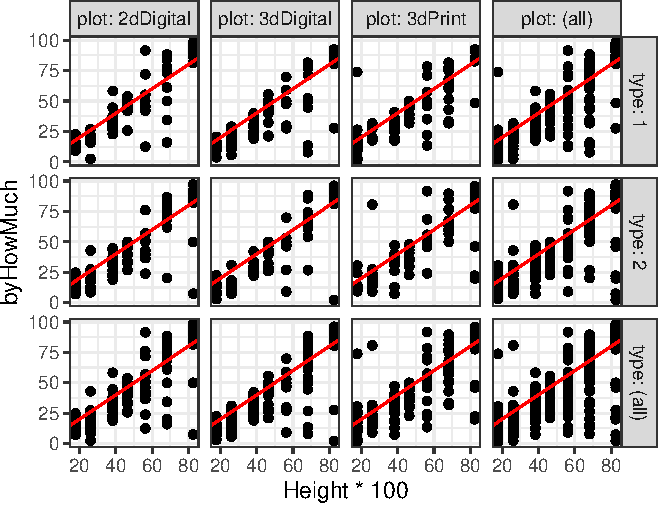
\includegraphics{index_files/figure-pdf/fig-ch1-raw-1.pdf}

}

\caption{\label{fig-ch1-raw}Responses of Project 1f}

\end{figure}%

\subsection{Project 1}\label{project-1-3}

\begin{Shaded}
\begin{Highlighting}[]
\NormalTok{pilot }\OtherTok{\textless{}{-}} \FunctionTok{read.csv}\NormalTok{(}\StringTok{\textquotesingle{}../ch1{-}bar3d/writeups/\_data/paper{-}data.csv\textquotesingle{}}\NormalTok{) }\SpecialCharTok{\%\textgreater{}\%} 
  \FunctionTok{filter}\NormalTok{(type }\SpecialCharTok{!=} \StringTok{"NA"}\NormalTok{)}
\FunctionTok{ggplot}\NormalTok{(pilot, }\FunctionTok{aes}\NormalTok{(}\AttributeTok{x =}\NormalTok{ Height}\SpecialCharTok{*}\DecValTok{100}\NormalTok{, }\AttributeTok{y =}\NormalTok{ response)) }\SpecialCharTok{+} 
  \FunctionTok{geom\_point}\NormalTok{() }\SpecialCharTok{+} 
  \FunctionTok{facet\_grid}\NormalTok{(type }\SpecialCharTok{\textasciitilde{}}\NormalTok{ plot, }\AttributeTok{margins =}\NormalTok{ T, }\AttributeTok{labeller =} \StringTok{\textquotesingle{}label\_both\textquotesingle{}}\NormalTok{) }\SpecialCharTok{+} 
  \FunctionTok{theme\_bw}\NormalTok{() }\SpecialCharTok{+} 
  \FunctionTok{theme}\NormalTok{(}\AttributeTok{aspect.ratio =} \DecValTok{1}\SpecialCharTok{/}\DecValTok{1}\NormalTok{)}
\end{Highlighting}
\end{Shaded}

\begin{figure}[H]

\centering{

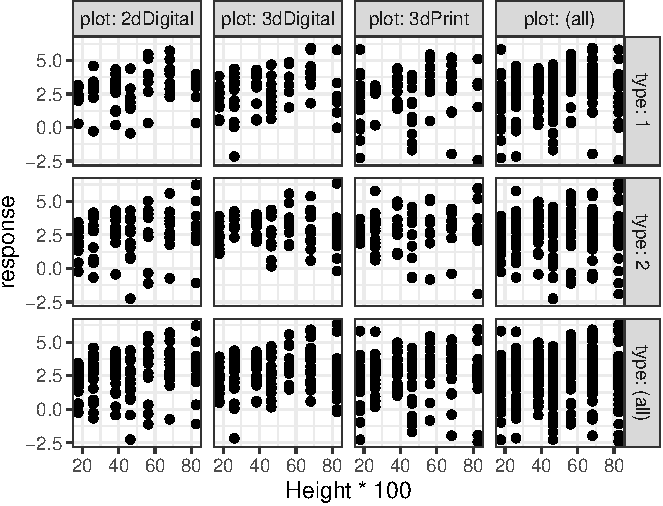
\includegraphics{index_files/figure-pdf/fig-ch1-logcm-1.pdf}

}

\caption{\label{fig-ch1-logcm}Responses of Project 1 using
log2(\textbar Error\textbar{} + 1/8)}

\end{figure}%

\subsection{Project 1}\label{project-1-4}

With estimates from the pilot study, a power analysis can be conducted.
Note that 18 out of 21 total kits were used in the analysis of the pilot
study.

\begin{itemize}
\item
  Power \textgreater{} 0.8 for ratio with 1 subject / kit
\item
  Power \textgreater{} 0.8 for plot(ratio) with 2 subjects / kit
\item
  Power \textgreater{} 0.8 for chart type with 17 subjects / kit
\item
  \(n=1\) per kit: Power \textgreater{} 0.8 for ratio of 46.4 between
  3dd and 3dp
\item
  \(n=10\) per kit: Power \textgreater{} 0.8 for 5/21 plot(ratio)
  comparisons
\item
  \(n=20\) per kit: Power \textgreater{} 0.8 for 11/21 plot(ratio)
  comparisons
\item
  \(n=40\) per kit: Power \textgreater{} 0.8 for 13/21 plot(ratio)
  comparisons
\end{itemize}

Power is low when the ratio is 17.8 and 56.2. Also note that \(n=40\)
per kit equates to \(840\) total subjects across 21 kits, which is
reasonable given the number of Stat 218 students enrolled across
multiple semesters.

\subsection{Project 3}\label{project-3}

What is the benefit of using the same ratio twice?

\begin{Shaded}
\begin{Highlighting}[]
\NormalTok{stimuli }\SpecialCharTok{\%\textgreater{}\%} 
  \FunctionTok{mutate}\NormalTok{(}\AttributeTok{diff =} \FunctionTok{round}\NormalTok{(}\FunctionTok{map2\_dbl}\NormalTok{(values, constant, \textbackslash{}(x,y)(}\FunctionTok{max}\NormalTok{(x,y)}\SpecialCharTok{{-}}\FunctionTok{min}\NormalTok{(x,y))),}\DecValTok{1}\NormalTok{),}
         \AttributeTok{ratio =} \FunctionTok{round}\NormalTok{(}\FunctionTok{map2\_dbl}\NormalTok{(values, constant, \textbackslash{}(x,y)(}\FunctionTok{min}\NormalTok{(x,y)}\SpecialCharTok{/}\FunctionTok{max}\NormalTok{(x,y))), }\DecValTok{2}\NormalTok{),}
         \AttributeTok{constant.in.pair =} \FunctionTok{case\_when}\NormalTok{(}
\NormalTok{           values }\SpecialCharTok{==}\NormalTok{ constant }\SpecialCharTok{\textasciitilde{}} \StringTok{\textquotesingle{}Stimuli are same value\textquotesingle{}}\NormalTok{,}
\NormalTok{           values }\SpecialCharTok{\textless{}}\NormalTok{ constant }\SpecialCharTok{\textasciitilde{}} \StringTok{\textquotesingle{}Constant is larger\textquotesingle{}}\NormalTok{,}
\NormalTok{           values }\SpecialCharTok{\textgreater{}}\NormalTok{ constant }\SpecialCharTok{\textasciitilde{}} \StringTok{\textquotesingle{}Constant is smaller\textquotesingle{}}
\NormalTok{         )) }\SpecialCharTok{\%\textgreater{}\%} 
  \FunctionTok{ggplot}\NormalTok{(}\FunctionTok{aes}\NormalTok{(}\AttributeTok{x =}\NormalTok{ ratio, }\AttributeTok{y =}\NormalTok{ diff, }\AttributeTok{color =}\NormalTok{ constant.in.pair)) }\SpecialCharTok{+} 
  \FunctionTok{geom\_point}\NormalTok{() }\SpecialCharTok{+} 
  \FunctionTok{scale\_color\_viridis\_d}\NormalTok{(}\AttributeTok{option =} \StringTok{\textquotesingle{}H\textquotesingle{}}\NormalTok{) }\SpecialCharTok{+}
  \FunctionTok{labs}\NormalTok{(}\AttributeTok{x =} \StringTok{\textquotesingle{}Ratio of stimuli\textquotesingle{}}\NormalTok{,}
       \AttributeTok{y =} \StringTok{\textquotesingle{}Difference of stimuli\textquotesingle{}}\NormalTok{,}
       \AttributeTok{color =} \StringTok{\textquotesingle{}Stimuli status\textquotesingle{}}\NormalTok{) }\SpecialCharTok{+} 
  \FunctionTok{theme\_bw}\NormalTok{() }\SpecialCharTok{+} 
  \FunctionTok{theme}\NormalTok{(}\AttributeTok{aspect.ratio =} \DecValTok{1}\NormalTok{)}
\end{Highlighting}
\end{Shaded}

\begin{figure}[H]

\centering{

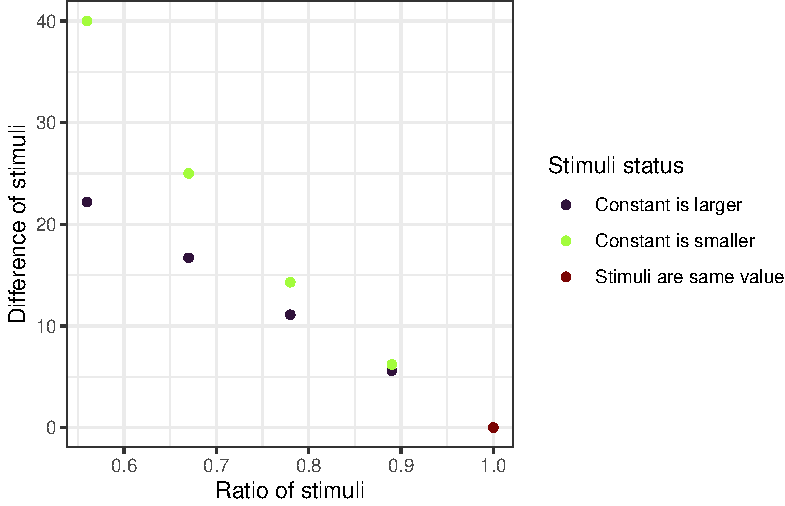
\includegraphics{index_files/figure-pdf/fig-diff-ratio-1.pdf}

}

\caption{\label{fig-diff-ratio}Scatterplot of ratios and difference of
each stimuli pairs.}

\end{figure}%

Since color does not have a direct translation to height, it is a good
idea to see if ratio estimations are different depending on the physical
different of the bars on the heat map.

Using the method of constant stimuli, stimuli pairs have a larger
difference for smaller ratios.

\begin{itemize}
\tightlist
\item
  If there is a difference in ratio estimations between stimuli pairs at
  the same ratio, then we show that the physical difference is also an
  important factor, meaning that future studies need to take this into
  consideration
\end{itemize}




\end{document}
